\documentclass[a5paper, oneside]{book}

%------кодировка и язык-------
\usepackage[T2A]{fontenc}
\usepackage[utf8]{inputenc}  
\usepackage[russian]{babel}

%-----------рисунки-----------
\usepackage{graphicx}   %графика
\usepackage{float}
\graphicspath{{pics/}}   %папка с картинками
\usepackage[left=1.5cm,right=1.5cm,bottom=2cm]{geometry} %настройка полей
\usepackage{subcaption}   %несколько фрагментов на рисунке

%--------векторная графика------
\usepackage{tikz}  % графика
\usepackage{circuitikz} % рисунки электических цепей
\usepackage{standalone}
\usetikzlibrary{patterns, angles, quotes, snakes}

%-----------формулы-----------
\usepackage{amsmath}
\usepackage{amssymb}
\usepackage[mathscr]{eucal} % шрифт в формулах для 

\usepackage{indentfirst} %отступ в первом абзаце

%------Формат заголовков глав---
\usepackage{titlesec}
\titleformat{\chapter}[display]{\normalfont\huge\bfseries}{}{0pt}{\Huge}
\titlespacing*{\chapter}{0pt}{10pt}{40pt}
\renewcommand*\thesection{\arabic{section}}
%\DeclareMathOperator{\tg}{tg}
\headsep=3mm   %расстояние между верхним колонтитулом и текстом

%----Условия, решения и ответы печатаются в разных частях документа---
\usepackage{answers} 
\Newassociation{sol}{Solution}{solutions}
\Newassociation{ans}{Answer}{answers}
\renewcommand{\Solutionlabel}[1]{\bf{Решение #1}}
\newtheorem{Exc}{Задача}
\newenvironment{ex}{\begin{Exc}\normalfont}{\end{Exc}}
\pagestyle{plain}

%-------------Секции по сложности задач--------------
\newcommand{\introProblems}{\subsection*{Задачи для разбора}}
\newcommand{\qualProblems}{\subsection*{Качественные задачи}}
\newcommand{\simpleProblems}{\subsection*{Задачи базового уровня}}
\newcommand{\complexProblems}{\subsection*{Задачи повышенного уровня}}

\begin{document}

\begin{titlepage}
	\centering
	
\includegraphics[width=0.15\textwidth]{logo.png}\par\vspace{1cm}
	{\scshape Пермский государственный национальный исследовательский университет\par}
	\vspace{0.5cm}
	{\scshape Физический факультет \par}
	\vspace{1cm}
	{\scshape\LARGE Задачи по механике\par}
	\vspace{2cm}
	{\Large\itshape К.А. Гаврилов\par}
	\vfill
	{\large \today\par}
\end{titlepage}

\tableofcontents    % Оглавление

\Opensolutionfile{solutions}[solutionsFile]
\Opensolutionfile{answers}[answersFile]

\chapter*{Предисловие}
\addcontentsline{toc}{chapter}{Предисловие} 
Методическое пособие включает в себя физические задачи, которые предлагаются для решения студентам 1 курса физического факультета Пермского государственного национального исследовательского университета при изучении курса "Механика". Выбранные задачи базового и повышенного уровня сложности предназначены для решения на практических занятиях, консультациях, а также для самостоятельного решения студентами.

\chapter*{Условия задач}
\addcontentsline{toc}{chapter}{Условия задач}
\section{Кинематика прямолинейного движения материальной точки}

\introProblems

\begin{ex} %ПодОл2-6
Координата движущейся по прямой точки меняется по закону: $x = 2 + 10t + 3t^2$ ($x$ измеряется в метрах, $t$ в секундах). Какова ее скорость при $t = 2$ с?
\begin{ans}
$v = 22$ м/с.
\end{ans}
\end{ex}

\begin{ex} %ПодОл2-7
Показать, что средняя скорость за промежуток времени от $t_1$ до $t_2$ при равноускоренном движении равна скорости в момент времени $(t_1 + t_2)/2$.
\end{ex}

\begin{ex} %ПодОл2-9 
От движущегося поезда отцепляют последний вагон. Поезд продолжает движение с той же скоростью $v_0$. Как будут относиться пути, пройденные поездом и вагоном к моменту остановки вагона? Считать, что вагон движется равнозамедленно. Решить задачу аналитически и графически.
\begin{ans}
2.
\end{ans}
\end{ex}

\begin{ex} %ПодОл2-13
Машинист пассажирского поезда, двигавшегося со скоростью $v_1 = 108$ км/ч, заметил на расстоянии $S_0 = 180$ м впереди движущийся в ту же сторону со скоростью $v_2 = 32,4$ км/ч товарный поезд. Машинист сразу включил тормоз, благодаря чему пассажирский поезд начал двигаться с ускорением $a = -1,2$ м/с\textsuperscript{2}. Достаточно ли этого ускорения для того, чтобы поезда не столкнулись?
\begin{ans}
Нет.
\end{ans}
\end{ex}

\begin{ex} %ПодОл2-18
За последнюю секунду свободно падающее тело прошло $3/4$ всего пути. С какой высоты оно упало?
\begin{ans}
20 м.
\end{ans}
\end{ex}

\qualProblems

\begin{ex} %Morin
Тело движется с отрицательной скоростью и отрицательным ускорением. Разгоняется ли оно при этом или тормозит?
\begin{ans}
Разгоняется.
\end{ans}
\end{ex}

\begin{ex} %Morin
На первом фрагменте рис. \ref{kinemInflection} изображён график зависимости ускорения материальной точки от времени, на втором рисунке изображена зависимость скорости другого тела от времени, на третьем рисунке – координата от времени. В каких из 12 изображённых точках ускорение обращается ноль? Все графики относятся к разным движущимся телам.

\begin{figure}[h]
\centering
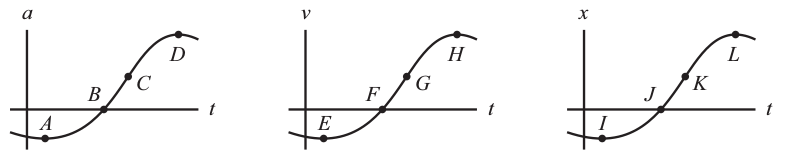
\includegraphics[width=0.8\textwidth]{kinemInflection.png}
\caption{}
\label{kinemInflection}
\end{figure}
\begin{ans}
$B, E, H, K$
\end{ans}
\end{ex}

\begin{ex} %Mproblems
При скатывании шарика вдоль наклонной плоскости без начальной скорости расстояния пройденный телом за одну, две, три секунды движения относятся как 1:4:9. Почему? Как относятся пути, пройденный шариком, в течение 1-ой секунды, 2-ой секунды, 3-ей секунды?
\begin{ans}
1:3:5
\end{ans}
\end{ex}

\begin{ex} %Mproblems
Как лучше поступить водителю, который подъезжает с максимальной разрешенной скоростью к перекрестку, на котором загорелся желтый сигнал светофора: затормозить или разогнаться, чтобы "проскочить" перекресток?
\end{ex}


\simpleProblems

\begin{ex} %Сив14
Начертить графики зависимости от времени скорости некоторых тел, если графики ускорения $a$ этих тел имеют вид, представленный на рис. \ref{kinemGraph} (начальная скорость тел во всех случаях равна нулю).

\begin{figure}[h]
\centering
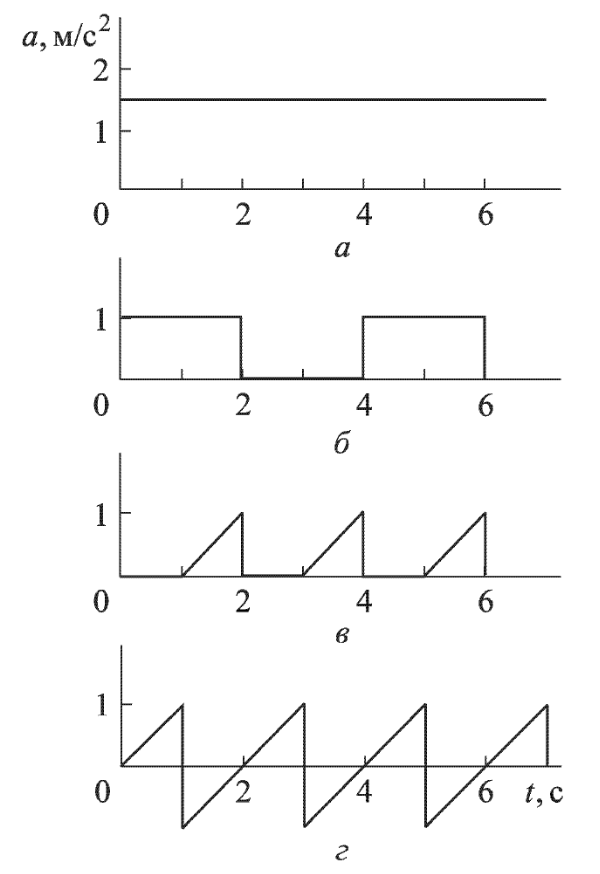
\includegraphics[width=0.45\textwidth]{kinemGraph.png}
\caption{}
\label{kinemGraph}
\end{figure}
\end{ex}

\begin{ex} %ПодОл2-34
Трамвай тормозит с постоянным ускорением до полной остановки. Найдите тормозной путь трамвая, если торможение заняло 5 с, а скорость трамвая на середине тормозного пути была 4 м/с.
\begin{ans}
$S = vt/\sqrt{2} = 14$ м.
\end{ans}
\end{ex}

\begin{ex} %Сив17
С вышки одновременно брошены два тела с одинаковой начальной скоростью $v_0$: одно вертикально вверх, другое вертикально вниз. Как с течением времени будет меняться расстояние $S$ между этими телами? Сопротивление воздуха движению тел не учитывать.
\begin{ans}
$S = 2 v_0 t$.
\end{ans}
\end{ex}

\begin{ex} %Сив33
Из точки, лежащей на верхнем конце вертикального диаметра некоторой окружности, по желобам, установленным вдоль различных хорд этой окружности, одновременно начинают скользить без трения грузы. Показать, что все грузы достигнут окружности одновременно.
\begin{ans}
$t = \sqrt{2D/g}$.
\end{ans}
\end{ex}

\begin{ex} %Сив15
Начертить графики зависимости от времени пути и ускорения некоторого тела, если скорость этого тела как функция времени представлена графиком на рис. \ref{kinemGraphAccel}.

\begin{figure}
\centering
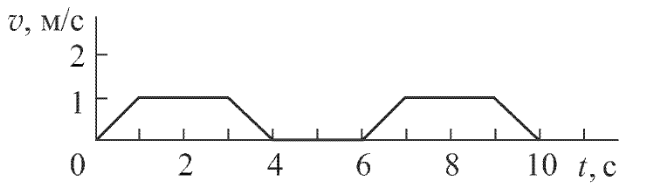
\includegraphics[width=0.6\textwidth]{kinemGraphAccel.png}
\caption{}
\label{kinemGraphAccel}
\end{figure}
\end{ex}

\begin{ex} %ПодОл2-19
С каким ускорением движется тело, если за восьмую секунду после начала прямолинейного движения оно прошло путь 30 м.
\begin{ans}
4 м/с\textsuperscript{2}.
\end{ans}
\end{ex}


\begin{ex} %ПодОл2-44
С высоты $H$ на упругую горизонтальную плиту свободно падает шарик. Построить график изменения координаты, скорость и ускорения шарика в зависимость от времени, считая, что временем соударения и сопротивлением воздуха можно пренебречь. Удар абсолютно упругий.
\end{ex}

\begin{ex} %Чертов1.21
Тело, брошенное вертикально вверх, находилось на одной и той же высоте $h = 8,6$ м два раза с интервалом $\Delta t = 3$ с. Пренебрегая сопротивлением воздуха, вычислить начальную скорость брошенного тела.
\begin{ans}
19,6 м/c
\end{ans}
\end{ex}

\begin{ex} %Чертов1.22
С балкона бросили мячик вертикально вверх с начальной скоростью $v_0 = 5$ м/с. Через $t = 2$ с мячик упал на землю. Определить высоту балкона над землей и скорость мячика в момент удара о землю.
\begin{ans}
9,62 м; 14,6 м/c
\end{ans}
\end{ex}

\complexProblems

\begin{ex} %Сив13
Тело, двигаясь с постоянным ускорением, проходит последовательно два одинаковых отрезка пути $S$ по 10 м каждый. Найти ускорение тела $a$ и скорость $v_0$ в начале первого отрезка, если первый отрезок пройден телом за время $t_1 = 1,06$ с, а второй за $t_2 = 2,2$ с.
\begin{ans}
$a = \frac{2S\left(t_1-t_2\right)}{t_1t_2\left(t_1+t_2\right)} \approx -3$ м/c\textsuperscript{2} , $v_0 = \frac{S}{t_1}-\frac{at_1}{2} \approx 11,5$ м/с.
\end{ans}
\end{ex}

\begin{ex} %ПодОл2-50
Муравей бежит от муравейника по прямой так, что его скорость обратно пропорциональна расстоянию до центра муравейника. В тот момент, когда муравей находится в точке $А$ на расстоянии 1 м от центра муравейника, его скорость равна 2 м/c. За какое время муравей добежит от точки А до точки $B$, которая находится на расстоянии 2 м от центра муравейника?
\begin{ans}
0,75 с.
\end{ans}
\end{ex}

\clearpage
\section{Движение тела, брошенного под углом к горизонту}

\introProblems

\begin{ex} %Сив21
Из артиллерийского орудия произведен выстрел под углом $\varphi$ к горизонту. Величина начальной скорости снаряда $v_0$. Исследовать аналитически движение снаряда, пренебрегая сопротивлением воздуха полету снаряда и кривизной поверхности Земли. Найденные зависимости изобразить графически. Найти: 1) вертикальную и горизонтальную компоненты вектора скорости $\vec{v}$ и абсолютную величину скорости как функцию времени; 2) время $Т$ полета снаряда от орудия до падения на землю; 3) зависимость от времени угла $\alpha$ между вектором скорости снаряда и горизонтом; 4) декартовы координаты (ось $X$ — горизонтальное направление, ось $Y$ — вертикальное направление) снаряда как функции времени; 5) уравнение траектории снаряда $y = f(x)$ (построить согласно этому уравнению траекторию полета снаряда); 6) максимальную высоту $H_{max}$ полета снаряда над землей; 7) горизонтальную дальность $L_{max}$ полета снаряда как функцию его начальной скорости и угла возвышения орудия; 8) При каком угле возвышения $\varphi^*$ дальность будет максимальной при заданной начальной скорости снаряда?
\begin{ans}
1) $v_x = v_0 \cos \varphi$, $v_y = v_0 \sin \varphi - gt$, $v = \sqrt{v_{0}^{2} + g^2 t^2 - 2v_{0}gt \sin \varphi}$; 2) $T = \frac{2v_{0}\sin \varphi}{g}$; 3) $ \tg \alpha = \tg \varphi - \frac{gt}{v_0 \cos \varphi}$; 4) $x = v_0 t \cos \varphi$, $y = v_0 t \sin \varphi - \frac{gt^2}{2}$; 5) $y = x \tg \varphi - \frac{gx^2}{2v_{0}^{2} \cos^2 \varphi} $; 6) $H_{\max} = \frac{v_{0}^{2} \sin^2 \varphi}{2g}$; 7) $L_{\max} = v_{0}^2 \sin 2 \varphi / g$; 8) $\varphi^{*} = 45^{\circ}$.
\end{ans}
\end{ex}	

\begin{ex} %Сив30
Самолет летит на высоте $h$ горизонтально по прямой со скоростью $v$. Летчик должен сбросить бомбу в цель, лежащую впереди самолета. Под каким углом $\alpha$ к вертикали он должен видеть цель в момент выпуска бомбы? Каково в этот момент расстояние $l$ от цели до точки, над которой находится самолет? Сопротивление воздуха движению бомбы не учитывать.
\begin{ans}
$\tg \alpha = v \sqrt{2/hg}$, $l = v \sqrt{2h/g}$.
\end{ans}
\end{ex}	

\begin{ex} %Иродов1.10
Два тела бросили одновременно из одной точки: одно — вертикально вверх, другое - под углом $\alpha = 60^{\circ}$ к горизонту. Начальная скорость каждого тела $v_0 = 25$ м/с. Найти расстояние между телами через $t = 1,70$ с.
\begin{ans}
$l = v_0 t \sqrt{2(1-\sin \alpha)} = 22$ м.
\end{ans}
\end{ex}	

\begin{ex} %Сив32
Цель, находящаяся на холме, видна с места расположения орудия под углом $\alpha$ к горизонту. Дистанция (расстояние по горизонтали от орудия до цели) равна $L$. Стрельба по цели производится при угле возвышения $\beta$. Определить начальную скорость $v_0$ снаряда, попадающего в цель. Сопротивление воздуха не учитывать.
\begin{ans}
$v_0 = \sqrt{\frac{lg \cos \alpha}{2 \cos \beta \sin \left( \beta - \alpha \right)}}$.
\end{ans}
\end{ex}	

\qualProblems
\begin{ex} %Марон
В каком случае выброшенная из вагона вещь долетит до земли раньше -- когда вагон покоится или когда он движется?
\begin{ans}
За одинаковое время.
\end{ans}
\end{ex}	

\begin{ex} %Morin
Камень брошен под углом к горизонту. Существует ли такое положение в процессе движения, в котором скорость перпендикулярна ускорению камня?
\begin{ans}
Верхняя точка траектории.
\end{ans}
\end{ex}	

\begin{ex} %Morin
Неопытный охотник бросает камень в обезьяну, сидящую на дереве высотой $H$ на расстоянии $L$ по горизонтали от охотника, при этом направляет вектор начальной скорости $v_0$ в местоположение обезьяны. В момент броска камня обезьяна отпускает руки и начинает свободно падать с дерева без начальной скорости. При каком условии камень может настичь обезьяну? 
\begin{ans}
$v_0 > \sqrt{\frac{g(H^2+L^2)}{2H}}$.
\end{ans}
\end{ex}	

\simpleProblems

\begin{ex} %Сив18
Какой начальной скоростью $v_0$ должна обладать сигнальная ракета, выпущенная из ракетницы под углом $45^{\circ}$ к горизонту, чтобы она вспыхнула в наивысшей точке своей траектории, если время горения запала ракеты 6 с? Сопротивление воздуха движению ракеты не учитывать.
\begin{ans}
$v_0 = 82$ м/с.
\end{ans}
\end{ex}	

\begin{ex} %ПодОл3-1
Точка движется согласно уравнениям: $x = 2t + 6, y = t^2$. Проходит ли ее траектория через точку $x = 10, y = 10$? Найдите величину и направление ускорения точки?
\begin{ans}
Нет, $a = 2$ м/с\textsuperscript{2}.
\end{ans}
\end{ex}	

\begin{ex} %Сив23
Из трех труб, расположенных на земле, с одинаковой скоростью бьют струи воды: под углом в $60^{\circ}$, $45^{\circ}$ и $30^{\circ}$ к горизонту. Найти отношение наибольших высот $H$ подъема струй воды, вытекающих из каждой трубы, и отношение дальностей падения $L$ воды на землю. Сопротивление воздуха движению водяных струй не учитывать.
\begin{ans}
$H_1 : H_2 : H_3 = 3 : 2 : 1$; $L_1 : L_2 : L_3 = \sqrt{3} : 2 : \sqrt{3}$.
\end{ans}
\end{ex}	

\begin{ex} %ПодОл3-5
Под каким углом к горизонту надо бросить камень, чтобы дальность его полета была втрое больше максимальной высоты подъема?
\begin{ans}
$55,1^{ \circ }$.
\end{ans}
\end{ex}	

\begin{ex} %Сив24
На какое максимальное расстояние $L$ можно бросить мяч в спортивном зале высотой 8 м, если мяч имеет начальную скорость 20 м/с? Какой угол $\varphi$ с полом зала должен в этом случае составлять вектор начальной скорости мяча? Считать, что высота начальной точки траектории мяча над полом мала по сравнению с высотой зала. Мяч во время полета не должен ударяться о потолок зала. Сопротивлением воздуха полету мяча пренебречь.
\begin{ans}
$L \approx 40$ м, $\varphi \approx 38^{\circ}40^\prime$.
\end{ans}
\end{ex}	

\begin{ex} %ПодОл3-8 
Камень бросили с крутого берега реки вверх под углом $30^{\circ}$ к горизонту со скоростью $v_0 = 10$ м/с. С какой скоростью он упал в воду, если время полета $t = 2$ с?
\begin{ans}
17 м/с.
\end{ans}
\end{ex}	

\complexProblems

\begin{ex} %Иродов1.11
Два шарика бросили одновременно из одной точки в горизонтальном направлении в противоположные стороны со скоростями $v_1 = 3,0$ м/с и $v_2 = 4,0$ м/с. Найти расстояние между шариками в момент, когда их скорости окажутся взаимно перпендикулярными.
\begin{ans}
$l = (v_1 + v_2)\sqrt{v_1 v_2}/g = 2,5$ м.
\end{ans}
\end{ex}	

\begin{ex} %ПодОл3-13 
Утка летела по горизонтальной прямой с постоянной скоростью $u$. В нее бросил камень неопытный охотник, причем бросок был сделан без упреждения, т.е. в момент броска скорость камня $v$ была направлена как раз на утку под углом $\alpha$ к горизонту (рис. \ref{duckHunter}). На какой высоте летела утка, если камень все же попал в нее? С какой стороны камень ударил утку?

\begin{figure}
\centering
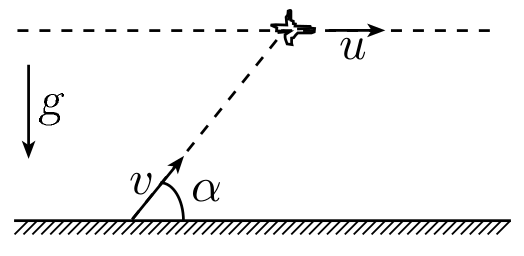
\includegraphics[width=0.4\textwidth]{duckHunter.png}
\caption{}
\label{duckHunter}
\end{figure}

\begin{ans}
$h = \frac{2u}{g}\left( v \cos \alpha - u \right) \tg^2 \alpha$.
\end{ans}
\end{ex}

\begin{ex} %Сив20
Шарик, которому сообщена горизонтальная скорость $v$, падает на горизонтальную плиту с высоты $h$. При каждом ударе о плиту вертикальная составляющая скорости уменьшается (отношение вертикальной составляющей скорости после удара к ее значению до удара
постоянно и равно $\alpha$). Определить, на каком расстоянии $х$ от места бросания отскоки шарика прекратятся. Считать, что трение отсутствует, так что горизонтальная составляющая скорости шарика $v$ не меняется
\begin{ans}
$x = v \sqrt{2h/g} \left( 1 + \alpha \right) / \left( 1 - \alpha \right)$.
\end{ans}
\end{ex}

\clearpage
\section{Кинематика вращательного движения материальной точки}

\introProblems

\begin{ex} %Сив43
Луна обращается вокруг Земли с периодом $T = 27,3$ сут относительно звезд. Средний радиус орбиты Луны $R = 3,8 \cdot 10^5$ км. Найти линейную скорость $v$ движения Луны вокруг Земли и ее нормальное ускорение $a$. 
\begin{ans}
$v = 2 \pi R/T = 3,7$ км/ч; $a = 4\pi^2 R/T^2 = 35$ км/ч\textsuperscript{2}.
\end{ans}
\end{ex}

\begin{ex} %Сив54
Якорь электромотора, вращавшегося с частотой $N$ оборотов в секунду, двигаясь после выключения тока равнозамедленно, остановился, сделав $n$ оборотов. Найти угловое ускорение якоря после выключения тока.
\begin{ans}
$\varepsilon = \pi N^2/n$.
\end{ans}
\end{ex}

\begin{ex} %Сив58
Автомобиль, движущийся со скоростью 40 км/ч, проходит закругление шоссе с радиусом кривизны 200 м. На повороте шофер тормозит машину, сообщая ей ускорение 0,3 м/с\textsuperscript{2}. Найти нормальное и полное ускорение автомобиля на повороте. Как направлен вектор полного ускорения $\vec{a}$ по отношению к радиусу кривизны $R$ закругления шоссе?
\begin{ans}
$a_n = 0.6$ м/с\textsuperscript{2}; $a = 0.67$ м/с\textsuperscript{2}; угол между векторами $\vec{a}$ и $\vec{R}$ составляет $135^{\circ}$.
\end{ans}
\end{ex}

\begin{ex} %Сив62
Колесо радиуса $R$ равномерно катится без скольжения по горизонтальному пути со скоростью $v$. Найти координаты $x$ и $y$ произвольной точки $A$ на ободе колеса, выразив их как функции времени $t$ или угла поворота колеса $\varphi$, полагая, что при $t = 0$ $\varphi = 0$, $x = 0$, $y = 0$ (рис. \ref{cycloid}). По найденным выражениям для $x$ и $y$ построить график траектории точки на ободе колеса.

\begin{figure}[h]
\centering
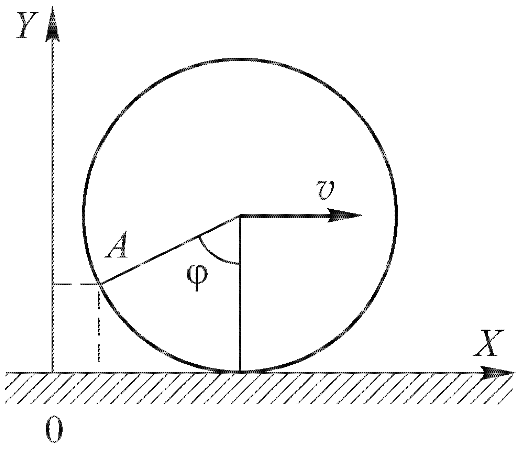
\includegraphics[width=0.3\textwidth]{cycloid.png}
\caption{}
\label{cycloid}
\end{figure}

\begin{ans}
$x= R(\varphi - \sin \varphi) = R(\omega t - \sin \omega t)$, $y=R(1-\cos \varphi) = R(1-\cos \omega t)$, где $\omega = v/R$ -- угловая скорость вращения колеса. Траекторией точек, находящихся на ободе движущегося колеса, будет простая циклоида.
\end{ans}
\end{ex}

\qualProblems

\begin{ex} %Сив44
Каковы будут графики зависимости от времени абсолютных величин скорости и ускорения при равномерном движении точки по кругу?
\end{ex}

\begin{ex} %Сив42
Точка движется равномерно по плоской траектории, изображенной на рис. \ref{maxAccel}. В каком месте траектории ускорение точки будет максимальным?

\begin{figure}[h]
\centering
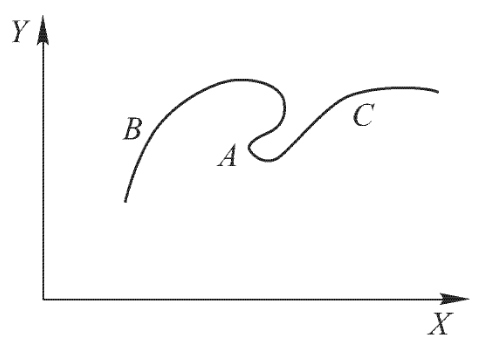
\includegraphics[width=0.4\textwidth]{maxAccel.png}
\caption{}
\label{maxAccel}
\end{figure}
\begin{ans}
A.
\end{ans}
\end{ex}

\begin{ex} %Сив44
Математический маятник отклонили на угол $\alpha = 45^{\circ}$ от положения равновесия и отпустили без начальной скорости. Под каким углом к горизонту направлен вектор ускорения маятника в начальный момент времени?
\begin{ans}
$90^{\circ}$.
\end{ans}
\end{ex}

\begin{ex}
Какую линию составляют концы векторов скорости материальной точки, равномерно вращающейся по окружности, если все векторы, соответствующие скорости снаряда в каждый момент времени, построить из одной точки. Искомый график называется годографом вектора скорости.
\begin{ans}
$90^{\circ}$.
\end{ans}
\end{ex}


\simpleProblems

\begin{ex} %Сив45
Найти среднюю угловую скорость искусственного спутника Земли, если период обращения его по орбите вокруг Земли составляет 105 мин.
\begin{ans}
$\omega \approx 0.001$ c\textsuperscript{-1}.
\end{ans}
\end{ex}

\begin{ex} %Сив49
Найти линейную скорость Земли, вызванную ее орбитальным движением. Средний радиус земной орбиты равен $R = 1.5 \cdot 10^8$ км.
\begin{ans}
$v \approx 30$ км/с.
\end{ans}
\end{ex}

\begin{ex} %Сив55
Автомобиль движется со скоростью 60 км/ч. Сколько оборотов в секунду делают его колеса, если они катятся по шоссе без скольжения, а внешний диаметр покрышек колес равен 60 см.
\begin{ans}
$\nu \approx 9$ об/с.
\end{ans}
\end{ex}

\begin{ex} %Сив57
Разматывая веревку и вращая без скольжения вал ворота, ведро опускается в колодец с ускорением 1 м/с\textsuperscript{2}. С каким угловым ускорением вращается вал ворота? Как зависит от времени угол поворота вала? Радиус вала ворота равен 25 см.
\begin{ans}
$\varepsilon = 4$ рад/c\textsuperscript{2}; $\varphi = 2t^2$ рад.
\end{ans}
\end{ex}

\begin{ex} %Чертов1.56
Маховик начал вращаться равноускоренно с за промежуток времени $t=10$ с достиг частоты вращения $n=300$ об/мин. Определите угловое ускорение $\varepsilon$ маховика и число оборотов $N$, которое он сделал за это время.
\begin{ans}
$\varepsilon =  3.14$ рад/\textsuperscript{2}, $N = 25$.
\end{ans}
\end{ex}

\begin{ex} %Чертов1.49
Тело брошено под углом $\alpha = 30^{\circ}$ к горизонту. Найти тангенциальное и нормальное ускорения в начальный момент движения.
\begin{ans}
5 м/c\textsuperscript{2}, 8.7 м/c\textsuperscript{2}.
\end{ans}
\end{ex}

\begin{ex} %Сив66
Представление о величине и направлении вектора полного ускорения при ускоренном вращательном движении (например, для точек якоря электромотора при его пуске) можно получить, рассмотрев следующую задачу. Точка движется по окружности радиусом $R$ с постоянным тангенциальным ускорением $a_{\tau}$, но без начальной скорости. Найти нормальное и полное ускорения точки, выразив их: 1) как функцию от времени $t$ и ускорения $a_{\tau}$; 2) как функцию от углового ускорения $\varepsilon$ и угла поворота $\varphi$ радиуса-вектора точки из его начального положения. Найти угол $\beta$ между направлением вектора полного ускорения точки и ее
радиусом-вектором.
\begin{ans}
$a_n = \frac{a_{\tau}^2 t^2}{R} = 2 \varepsilon R \varphi$; $a = \frac{a_{\tau}}{R} \sqrt{R^2 + a_{\tau}^2 t^4} = \varepsilon R \sqrt{1 + 4 \varphi^2}$; $\tg \beta = -\frac{1}{2\varphi}$.
\end{ans}
\end{ex}

\complexProblems

\begin{ex} %Сив59
Колесо радиуса $R$ катится без скольжения по горизонтальной дороге со скоростью $v_0$ (рис. \ref{rollingWheel}). Найти горизонтальную компоненту $v_x$ линейной скорости движения произвольной точки на ободе колеса, вертикальную компоненту $v_y$ этой скорости и модуль полной скорости для этой же точки. Найти значение угла $\alpha$ между вектором полной скорости точек на ободе колеса и направлением поступательного движения его оси. Показать, что направление вектора полной скорости произвольной точки $A$ на ободе колеса всегда перпендикулярно к прямой $AB$ и проходит через высшую точку катящегося колеса. Показать, что для точки $A$: $v = BA \omega$. Построить график распределения скоростей для всех точек на вертикальном диаметре (в данный момент времени) катящегося без скольжения колеса. Выразить все искомые величины через $v_0$, $R$ и угол $\varphi$, составленный верхним вертикальным радиусом колеса и радиусом, проведенным из центра колеса $O$ в исследуемую точку его обода $A$.

\begin{figure}[h]
\centering
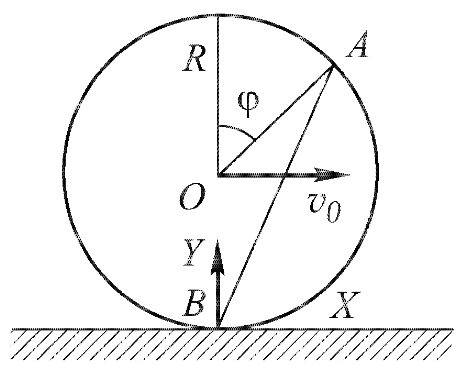
\includegraphics[width=0.4\textwidth]{rollingWheel.png}
\caption{}
\label{rollingWheel}
\end{figure}

\begin{ans}
$v_x = v_0 (1 + \cos \varphi) = 2v_0 \cos^2 \frac{\varphi}{2}$; $v_y = -v_0 \sin \varphi$; $v = 2v_0 \cos \frac{\varphi}{2}$.
\end{ans}
\end{ex}

\begin{ex} %Сив64
Автомобиль с колесами радиуса $R$ движется со скоростью $v$ по горизонтальной дороге, причем $v^2 > Rg$, где $g$ -- ускорение свободного падения. На какую максимальную высоту $H_{\max}$ может быть заброшена вверх грязь, срывающаяся с колес автомобиля? Указать положение той точки на покрышке колеса, с которой при данной скорости движения автомобиля грязь будет забрасываться выше всего. Сопротивление воздуха движению отброшенной вверх грязи не учитывать.
\begin{ans}
$H_{\max} = R + \frac{v^2}{2g} + \frac{gR^2}{2v^2}$; $\cos \varphi^{*} = - \frac{Rg}{v^2}$.
\end{ans}
\end{ex}

\begin{ex} %Иродов1.57

\begin{figure}[h]
\centering
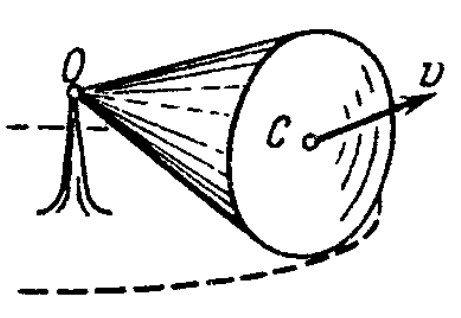
\includegraphics[width=0.4\textwidth]{rollingCylinder.png}
\caption{}
\label{rollingCylinder}
\end{figure}

Круглый конус с углом полураствора $\alpha = 30^{\circ}$ и радиусом основания $R = 5,0$ см катится равномерно без скольжения по горизонтальной плоскости, как показано на рис. \ref{rollingCylinder}. Вершина конуса закреплена шарнирно в точке $O$, которая находится на одном уровне с точкой $C$ -- центром основания конуса. Скорость точки $C$ равна $v = 10,0$ см/с. Найти модули: 1) угловой скорости конуса; 2) углового ускорения конуса.

\begin{ans}
1) $\omega = \frac{v}{R \cos \alpha} = 0,6$ рад/с; 2) $\varepsilon = (v/R)^2 \tg \alpha = 2,3$ рад/c\textsuperscript{2}.
\end{ans}
\end{ex}

\clearpage
\section{Динамика материальной точки}

\introProblems

\begin{ex} %Сив73
В лифте установлены пружинные весы, на которых подвешено тело массы 1 кг. Что будут показывать весы, если лифт: 1) движется вверх с ускорением 5 м/с\textsuperscript{2}, направленным вниз; 2) движется вниз с ускорением 5 м/с\textsuperscript{2}, направленным вверх?
\begin{ans}
1) 5 Н; 2) 15 Н.
\end{ans}
\end{ex}

\begin{ex} %Сив76
На гладкой горизонтальной плоскости находится тело массы $M$ (рис. \ref{block2Bodies}). Другое тело массы $m$ подвешено на нити, перекинутой через блок и привязанной к телу массы $M$. Найти ускорения тел и натяжение нити. Трением тела массы $М$ о плоскость и трением в блоке, а также массами блока и нити пренебречь.

\begin{figure}[h]
\centering
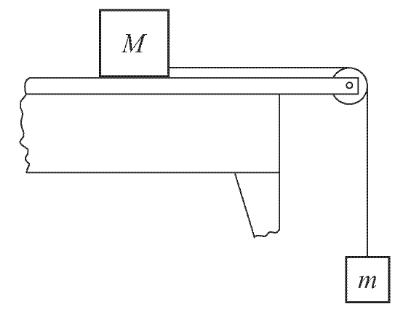
\includegraphics[width=0.45\textwidth]{block2Bodies.png}
\caption{}
\label{block2Bodies}
\end{figure}

\begin{ans}
$a = \frac{mg}{m+M}$; $T = \frac{mMg}{m+M}$.
\end{ans}
\end{ex}

\begin{ex} %Сив79
По наклонной плоскости с углом наклона $\alpha$ скользит тело. Сила трения между телом и плоскостью пропорциональна силе нормального давления тела на плоскость и не зависит от скорости тела. Коэффициент трения между трущимися поверхностями тела и плоскости равен $\mu$. Найти ускорение $a$, с которым скользит тело.
\begin{ans}
$a = g (\sin \alpha - \mu \cos \alpha)$, при $\tg \alpha > \mu$.
\end{ans}
\end{ex}

\begin{figure}[h]
\centering
\begin{subfigure}{.43\textwidth}
  \centering
  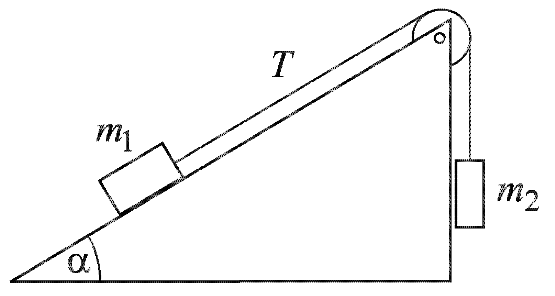
\includegraphics[width=1.0\linewidth]{inclinedPlane.png}
  \caption{}
  \label{inclinedPlane}
\end{subfigure}%
\begin{subfigure}{.57\textwidth}
  \centering
  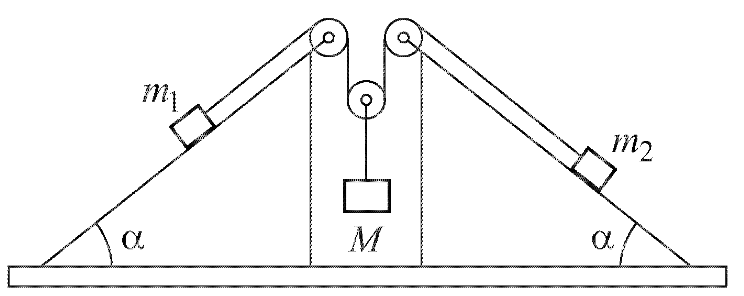
\includegraphics[width=1.0\linewidth]{2InclinedPlanes.png}
  \caption{}
  \label{2InclinedPlanes}
\end{subfigure}
\caption{}
\end{figure}

\begin{ex} %Сив96
На верхнем краю идеально гладкой наклонной плоскости укреплен блок, через который перекинута нить (рис. \ref{inclinedPlane}). На одном ее конце привязан груз с массой $m_1$, лежащий на наклонной плоскости. На другом конце висит груз с массой $m_2$. С каким ускорением $a$ движутся грузы и каково натяжение $Т$ нити? Наклонная плоскость образует с горизонтом угол $\alpha$.
\begin{ans}
$a = \frac{m_1 \sin \alpha - m_2}{m_1 + m_2}g$; $T = \frac{m_1 m_2}{m_1 + m_2}\left( 1+ \sin \alpha \right)g$.
\end{ans}
\end{ex}

\begin{ex} %Сив97
Определить ускорение массы $М$ в системе, изображенной на рис. \ref{2InclinedPlanes}. Массой блоков и силами трения можно пренебречь. Клинья считать закрепленными жестко.
\begin{ans}
$a = \frac{M(m_1 + m_2) - 4 m_1 m_2 \sin \alpha}{M(m_1 + m_2) + 4 m_1 m_2}g$.
\end{ans}
\end{ex}

\qualProblems

\begin{ex}
Надувной матрас заполнен воздухом до давления, превышающего атмосферное. В каком случае давление воздуха в матрасе будет больше: когда человек ляжет на него или когда встанет?
\end{ex}

\begin{ex} %Morin
Два человека тянут веревку в разные стороны, при этом каждый прикладывает силу $F$. Какова сила натяжения веревки?
\begin{ans}
$F$.
\end{ans}
\end{ex}

\begin{ex} %Morin
Два груза равной массы расположены один на другом и помещаются на горизонтальной гладкой поверхности. К нижнему грузу прикладывают горизонтальную силу $F$ и вся система начинает равноускоренно двигаться. Какая сила приводит в движение верхний груз?
\end{ex}

\begin{ex} %Morin
В салоне самолета, который разгонятся на взлетно-посадочной полосе, подвешен в равновесии математический маятник. Будет ли нить этого маятника располагаться вертикально?
\end{ex}

\begin{ex} %Morin
Когда водитель нажимает на педаль газа, автомобиль массы $m$ начинает разгоняться c ускорением $a$, причем $F = ma$, где $F$ - некоторая сила. Что за сила действуют на автомобиль при разгоне?
\end{ex}

\begin{ex} %Morin
Какие санки скатятся быстрее с горки -- с грузом или без груза? Почему?
\end{ex}

\simpleProblems

\begin{ex} %Сив78
На гладкую горизонтальную плоскость помещены три массы $m_1$, $m_2$, $m_3$ связанные нитями между собой и с массой $M$, привязанной к нити, перекинутой через блок (рис. \ref{4Bodies}). 1) Найти ускорение $a$ системы; 2) найти натяжение всех нитей. Трением тел о плоскость и трением в блоке, а также массами блока и нити пренебречь.
\begin{ans}
$a = \frac{Mg}{M + m_1 +m_2 +m_3}$, $T_1 = (m_1 +m_2 +m_3)a$, $T_2 = (m_2 +m_3)a$, $T_3 = m_3 a$.
\end{ans}
\end{ex}

\begin{figure}[h]
\centering
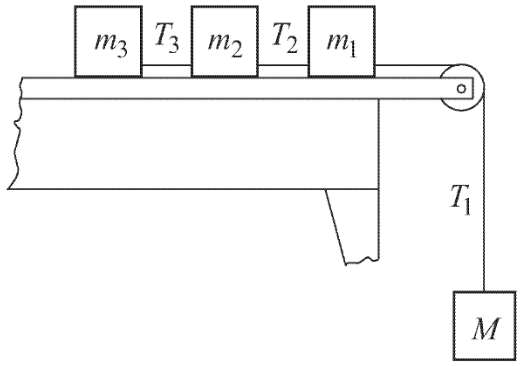
\includegraphics[width=0.5\textwidth]{4Bodies.png}
\caption{}
\label{4Bodies}
\end{figure}

\begin{ex} %Сив80
Два одинаковых тела связаны нитью и лежат на идеально гладком горизонтальном столе, так что нить представляет собой прямую линию. Нить может выдерживать натяжение с силой не более 100 Н. Какую горизонтальную силу $F$ следует приложить к одному из тел, чтобы нить оборвалась?
\begin{ans}
200 H.
\end{ans}
\end{ex}

\begin{ex}
Два бруска массами $m_1$ и $m_2$ расположены один на другом и помещаются на горизонтальной гладкой поверхности. Какую горизонтальную силу $F$ нужно приложить к нижнему грузу массой $m_2$, чтобы выдернуть его из-под верхнего? Коэффициент трения между брусками равен $\mu$.
\end{ex}

\begin{ex} %Сив85-86
Лошадь равномерно тянет сани. Рассмотреть взаимодействие трех тел: лошади, саней и поверхности земли. Начертить векторы сил, действующих на каждое из этих тел в отдельности. Найти величину всех сил, если лошадь и сани движутся с ускорением $a = 20$ см/с\textsuperscript{2}. Масса саней с грузом $M = 0,5$ т, масса лошади $m = 0,35$ т и коэффициент трения саней о снег $\mu = 0,2$.
\begin{ans}
На лошадь со стороны Земли действует сила $F = M(\mu g + a) + ma = 1,17$ кН.
\end{ans}
\end{ex}

\begin{ex} %Сив90
Воздушный шар массы $M$ опускается с постоянной скоростью. Какое количество балласта $m$ надо выбросить, чтобы шар начал подниматься с той же скоростью? Подъемную силу $Р$ шара считать постоянной.
\begin{ans}
$m = 2(M - P/g)$.
\end{ans}
\end{ex}

\begin{figure}[h]
\centering
\begin{subfigure}[t]{.3\textwidth}
  \centering
  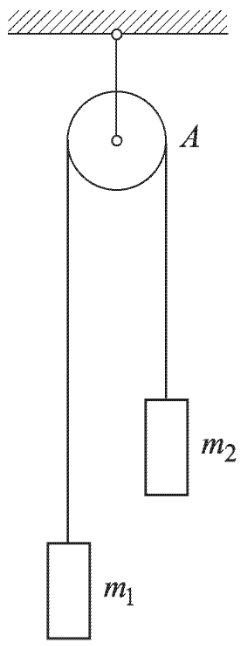
\includegraphics[width=0.7\linewidth]{Atwood.png}
  \caption{}
  \label{Atwood}
\end{subfigure}
\begin{subfigure}[t]{.3\textwidth}
  \centering
  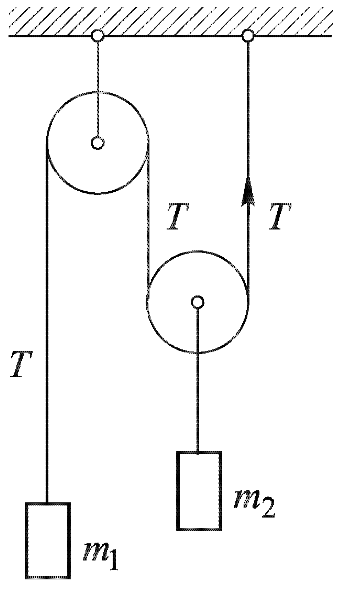
\includegraphics[width=1.0\linewidth]{Atwood2.png}
  \caption{}
  \label{Atwood2}
\end{subfigure}
\begin{subfigure}[t]{.3\textwidth}
  \centering
  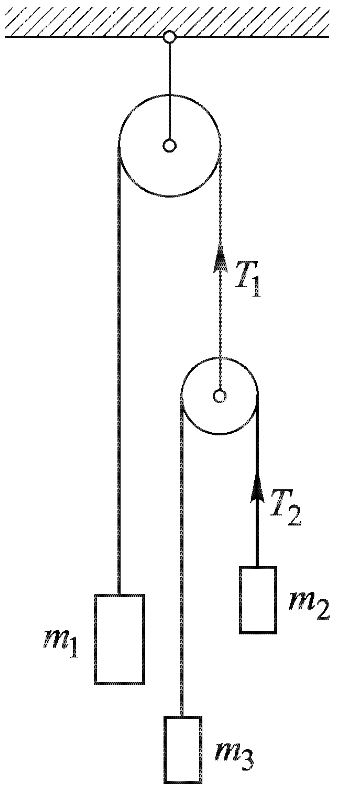
\includegraphics[width=1.0\linewidth]{Atwood3.png}
  \caption{}
  \label{Atwood3}
\end{subfigure}
\caption{}
\end{figure}

\begin{ex}
С вершины наклонной плоскости высотой 5 м и углом наклона к горизонту $45^{\circ}$ начинает соскальзывать тело. Определите скорость тела в конце спуска, если коэффициент трения тела  о плоскость равен 0,19.
\begin{ans}
$ v = \sqrt{2gh(1 - \mu \cot \alpha)} = 9 \textrm{ м/c}.$
\end{ans}
\end{ex}

\begin{ex} %Сив95
Простейшую машину Атвуда, служащую для проверки законов равноускоренного движения, можно схематически представить так: на нити, перекинутой через блок $A$, подвешены две неравные массы, $m_1$
и $m_2$ (рис. \ref{Atwood}). Найти ускорение масс, натяжение нити $T$ и силу $F$, действующую на ось блока этой машины. Блок и нить считать невесомыми, трения в оси блока не учитывать.
\begin{ans}
$a = (m_1 - m_2)g / (m_1 + m_2)$, $T = 2 m_1 m_2 g /(m_1 + m_2)$, $F = 2T$.
\end{ans}
\end{ex}

\begin{ex} %Сив103
Найти ускорения $a_1$ и $a_2$ масс $m_1$ и $m_2$ и натяжение нити $Т$ в системе, изображенной на рис. \ref{Atwood2}. Массой блоков и нитей пренебречь.
\begin{ans}
$a_1 = (2m_1-m_2)g/(2m_1+0,5m_2)$, $a_2 = -a_1/2$, $T=3m_1 m_2g/(4m_1 + m_2)$.
\end{ans}
\end{ex}

\complexProblems

\begin{ex} %Сив104
Найти ускорение массы $m_1$ и натяжения нитей $T_1$ и $T_2$ в системе, изображенной на рис. \ref{Atwood3}. Массой блоков и нитей пренебречь, сил трения не учитывать.
\begin{ans}
$a_1 = \frac{m_1(m_2+m_3)-4m_2m_3}{m_1(m_2+m_3)+4m_2m_3}g$, $T= \frac{8m_1m_2m_3g}{m_1(m_2+m_3)+4m_2m_3}$, $T_2 = T_1/2$.
\end{ans}
\end{ex}

\begin{ex} %Иродов1.65
Небольшое тело пустили вверх по наклонной плоскости, составляющей угол $\alpha  = 15^{\circ}$ с горизонтом. Найти коэффициент трения, если время подъема тела оказалось в $k = 2,0$ раза меньше времени спуска.
\begin{ans}
$\mu = \tg \alpha (k^2-1)/(k^2+1) = 0,16$.
\end{ans}
\end{ex}

\begin{ex} %Сив112
Как будет изменяться скорость тела массы $m$, движущегося вертикально вверх с начальной скоростью $v_0$, если можно считать, что сила сопротивления воздуха пропорциональна скорости тела $F = -rv$, где $r$ -- постоянный коэффициент сопротивления?
\begin{ans}
$v = \frac{mg}{r}\left[ \left( \frac{v_0r}{mg} +1 \right)e^{-\frac{rt}{m}} - 1 \right]$.
\end{ans}
\end{ex}

\clearpage
\section{Закон сохранения импульса}

\begin{ex} %Сив187
С какой скоростью $v$ после горизонтального выстрела из винтовки стал двигаться стрелок, стоящий на весьма гладком льду? Масса стрелка с винтовкой и снаряжением составляет 70 кг, а масса пули 10 г и ее начальная скорость 700 м/с.
\begin{ans}
$v=10$ см/с.
\end{ans}
\end{ex}

\begin{ex} %Сив188
Определить силу, с которой винтовка действует на плечо стрелка при выстреле, если считать, что со стороны винтовки действует постоянная сила и смещает плечо стрелка на $S = 1,5$ см, а пуля покидает ствол мгновенно. Масса винтовки 5 кг, масса пули 10 г, и скорость ее при вылете равна $v = 500$ м/с.
\begin{ans}
$F = \frac{m^2 v^2}{2SM}$
\end{ans}
\end{ex}

\begin{ex} %Сив191
Три лодки одинаковой массы $m$ идут в кильватер (друг за другом) с одинаковой скоростью $v$. Из средней лодки одновременно в переднюю и заднюю лодки бросают со скоростью $u$ относительно лодки грузы массы $m_1$. Каковы будут скорости лодок после переброски грузов?
\begin{ans}
$v_1 = \frac{m_1(v+u)+mv}{m+m_1}$, $v_2 = v$, $v_3 = \frac{m_1(v-u)+mv}{m+m_1}$.
\end{ans}
\end{ex}

\begin{ex} %Сив194
В шар массы $m_1$, движущийся со скоростью $v_1$, ударяется другой шар массы $m_2$, догоняющий первый в том же направлении со скоростью $v_2$. Считая удар абсолютно неупругим, найти скорости шаров после удара и их кинетическую энергию.
\begin{ans}
$v = \frac{m_1v_1 + m_2v_2}{m_1+m_2}$, $K = \frac{(m_1v_1+m_2v_2)^2}{2(m_1+m_2)}$.
\end{ans}
\end{ex}

\begin{ex} %Сив190
Снаряд разрывается в верхней точке траектории на высоте $h = 19,6$ м на две одинаковые части. Через секунду после взрыва одна часть падает на Землю под тем местом, где произошел взрыв. На каком расстоянии $S_2$ от места выстрела упадет вторая часть снаряда, если первая упала на расстоянии $S_1 = 1000$ м от места выстрела? Сил сопротивления воздуха при решении задачи не учитывать.
\begin{ans}
$S_2 = 5$ км.
\end{ans}
\end{ex}

\begin{ex} %Сив193
Две лодки идут навстречу параллельным курсом. Когда лодки находятся друг против друга, с каждой лодки во встречную перебрасывается мешок массой в 50 кг, в результате чего первая лодка останавливается, а вторая идет со скоростью 8,5 м/с в прежнем направлении. Каковы были скорости лодок до обмена мешками, если массы лодок с грузом равны 500 кг и 1 т соответственно?
\begin{ans}
9 м/с и 1 м/с.
\end{ans}
\end{ex}

\begin{ex} %Сив199
С какой скоростью $v$ должен лететь снаряд массы $m$ = 10 кг, чтобы при ударе о судно массы $М$ = 100 т последнее получило скорость $v_1$ = 0,1 м/с? Удар считать неупругим.
\begin{ans}
1 км/c.
\end{ans}
\end{ex}

\begin{ex} %Сив200
Ледокол, ударяясь о льдину массы $М$, отбрасывает ее, сообщив ей скорость $v$ [м/с]. Положим, что давление ледокола на льдину нарастает равномерно во времени при сближении ледокола со льдиной и также равномерно убывает, когда они расходятся. Найти при этих условиях максимальную силу давления льдины на борт корабля, если удар продолжался $\tau$ [с].
\begin{ans}
$F = 2Mv/\tau$.
\end{ans}
\end{ex}

\begin{ex} %Сив201
В одном изобретении предлагается на ходу наполнять платформы поезда углем, падающим вертикально на платформу из соответствующим образом устроенного бункера. Какова должна быть приложенная к платформе сила тяги, если на нее погружают 10 т угля за 2 с, и за это время она проходит равномерно 10 м? Трением при движении платформы можно пренебречь.
\begin{ans}
$F = \Delta m v/ \Delta t$.
\end{ans}
\end{ex}

\begin{ex} %Сив233
Лодка массы $M$ с находящимся в ней человеком массы $m$ неподвижно стоит на спокойной воде. Человек начинает идти вдоль по лодке со скоростью $\vec{u}$ и относительно лодки. С какой скоростью $\vec{w}$ будет двигаться человек относительно воды? С какой скоростью $\vec{v}$ будет при этом двигаться лодка относительно воды? Сопротивление воды движению лодки не учитывать.
\begin{ans}
$\vec{w} = \frac{M\vec{u}}{M+m}$, $\vec{v} = -\frac{m\vec{u}}{M+m}$.
\end{ans}
\end{ex}

\begin{ex} %Сив234
Пусть человек прошел вдоль по лодке, описанной в предыдущей задаче, его перемещение составило $\vec{l}$. Каковы будут при этом смещения лодки $\vec{S_1}$ и человека $\vec{S_2}$ относительно воды?
\begin{ans}
$\vec{S_1} = -\frac{m\vec{l}}{M+m}$, $\vec{S_2} = \frac{M\vec{l}}{M+m}$.
\end{ans}
\end{ex}

\begin{ex} %Иродов1.129
В момент, когда скорость падающего тела составила $v_0 = 4,0$ м/с, оно разорвалось на три одинаковых осколка. Два осколка разлетелись в горизонтальной плоскости под прямым углом друг к другу со скоростью $v = 5,0$ м/с каждый. Найти скорость третьего осколка сразу после разрыва.
\begin{ans}
$u = \sqrt{9v_{1}^2 + 2v^2} = 14$ м/с.
\end{ans}
\end{ex}

\begin{ex} %Иродов1.132
Цепочка массы $m = 1,00$ кг и длины $l = 1,40$ м висит на нити, касаясь поверхности стола своим нижним концом. После пережигания нити цепочка упала на стол. Найти полный импульс, который она передала столу.
\begin{ans}
$p = (2m/3)\sqrt{2gl} = 3,5$ кг$\cdot$м/c.
\end{ans}
\end{ex}

\begin{ex} %МФТИ3.5
С какой силой пожарный должен удерживать пожарный шланг, вода из которого выбрасывается в виде потока мелких капель в количестве $Q = 10$ кг/с и может добивать до высоты $h = 10$ м? Оцените, какая сила будет действовать на стену, если на нее направить струю из этого шланга под углом $45^{\circ}$ (оценку провести в двух предельных случаях -- для упругого и для неупругого соударения капель со стенкой).
\begin{ans}
$F_1 = Q\sqrt{2gh} \approx 140$ Н, $F_2 = \sqrt{2} F_1 \approx 200$ Н, $F_3 = F_1/\sqrt{2} \approx 100$ Н. 
\end{ans}
\end{ex}

\clearpage
\section{Работа. Закон сохранения энергии}

\introProblems

\begin{ex} %Сив162
Коэффициент трения между некоторым телом и плоскостью, наклоненной под углом $45^{\circ}$ к горизонту, равен 0,2. На какую высоту поднимается это тело, скользя по наклонной плоскости, если ему будет сообщена скорость 10 м/с, направленная вверх вдоль плоскости? Какова будет скорость тела, когда оно вернется в нижнюю исходную точку своего движения?
\begin{ans}
4,25 м; $\approx$ 8,16 м/с.
\end{ans}
\end{ex}

\begin{ex} %Сив166
Из залитого подвала, площадь пола которого равна 50 м\textsuperscript{2}, требуется выкачать воду на мостовую. Глубина воды в подвале 1,5 м, а расстояние от уровня воды в подвале до мостовой 5 м. Найти работу, которую необходимо затратить для откачки воды.
\begin{ans}
4,3 МДж.
\end{ans}
\end{ex}

\begin{ex} %Сив170
Определить среднюю полезную мощность при выстреле из гладкоствольного ружья, если известно, что пуля массы $m$ вылетает из ствола со скоростью $v_0$, а длина канала ствола $l$ (давление пороховых газов считать постоянным во все время нахождения снаряда в канале ствола).
\begin{ans}
$N =\frac{mv_{0}^3}{4l}$.
\end{ans}
\end{ex}


\begin{ex} %Сив196
На гладком горизонтальном столе лежит шар массы $m_1$, соединенный с пружиной жесткости $k$. Второй конец пружины закреплен (рис. \ref{2BallsSpring}). Происходит лобовое упругое соударение этого шара с другим шаром, масса которого $m_2$ меньше $m_1$, а скорость равна $v$. В какую сторону будет двигаться второй шар после удара? Определить амплитуду колебаний первого шара после соударения.

\begin{figure}[h]
\centering
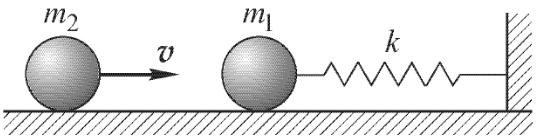
\includegraphics[width=0.5\textwidth]{2BallsSpring.png}
\caption{}
\label{2BallsSpring}
\end{figure}

\begin{ans}
После соударения второй шарик отскочит назад, $A = \frac{2m_2v}{m_1+m_2}\sqrt{\frac{m_1}{k}}$.
\end{ans}
\end{ex}

\begin{ex} %Сив227
Баллистический маятник — это маятник, употребляющийся для определения скорости снаряда. Принцип его действия заключается в том, что снаряд, скорость которого следует измерить, ударяется в тело маятника длины $l$ (рис. \ref{ballisticPendulum}). Если известны условия удара и массы снаряда $m$ и маятника $M$, то по углу отклонения маятника $\alpha$ можно вычислить скорость $v$ снаряда до удара. Показать, как это сделать для случая, когда снаряд после удара застревает в маятнике.

\begin{figure}[h]
\centering
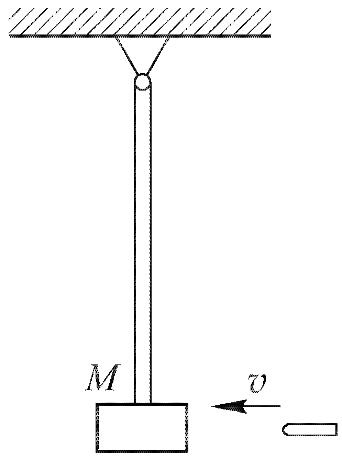
\includegraphics[width=0.25\textwidth]{ballisticPendulum.png}
\caption{}
\label{ballisticPendulum}
\end{figure}

\begin{ans}
$v = 2\frac{M+m}{m}\sqrt{lg}\sin \frac{\alpha}{2}$.
\end{ans}
\end{ex}

\qualProblems

\begin{ex}
Знак многих физических величин зависит от выбора системы координат, например, проекция ускорение сводного падения может быть положительной, если ось направить вниз, или отрицательной, если ось направить вверх. Может ли механическая работа подобным образом изменять знак в разных системах координат?
\end{ex}

\begin{ex}
Какая из следующих сил ни при каких обстоятельствах не совершает работу:
\begin{itemize}
\item гравитационная сила;
\item сила трения покоя;
\item сила трения скольжения;
\item сила натяжения;
\item сила реакции опоры.
\end{itemize}
\end{ex}

\begin{ex}
Эскалатор движется вниз с постоянной скорость. Вы поднимаетесь по эскалатору с такой же скоростью вверх, таким образом относительно земли остаетесь на месте. Совершаете ли Вы работу при этом?
\end{ex}

\begin{ex}
Веревку, привязанную к телу, тянут с постоянной силой, заставляя тело двигаться с постоянным ускорением. Согласно 3 закону Ньютона, тело действует на веревку с такой же по модулю силой в противоположном направлении. Будет ли суммарная работа этих сил равна нулю? Если да, то за счет какой работы увеличивается кинетическая энергия тела? 
\end{ex}

\begin{ex}
За счет изменения какой энергии воздушный шар поднимается вверх?
\end{ex}

\begin{ex}
Тело бросают под углом к горизонту под различными углами с одинаковой начальной скорость. Начальная кинетическая энергия во всех случаях одинакова, почему же различна высота подъема (максимальная потенциальная энергия)?
\end{ex}

\begin{ex}
Человек прыгает на батуте, при этом с каждым прыжком его максимальная высота подъема (потенциальная энергия) увеличивается. Трение о воздух, наоборот, должно приводить к уменьшению механической энергии системы. За счет чего растет энергия системы?
\end{ex}

\begin{ex}
Изобразите график зависимости потенциальной энергии гравитационного взаимодействия Земли и тела вблизи ее поверхности. Как использовать этот график для объяснения свободного тел на Землю?
\end{ex}

\begin{ex}
Может ли действие силы трения привести к увеличение механической энергии системы? Если да, приведите примеры. 
\end{ex}

\simpleProblems

\begin{ex} %Сив163
Какую работу надо совершить, чтобы втащить (волоком) тело массы $m$ на горку с длиной основания $L$ и высотой $H$, если коэффициент трения между телом и поверхностью горки равен $\mu$? Как изменится ответ, если угол наклона поверхности горки с горизонтом может меняться вдоль горки, но его знак остается постоянным.
\begin{ans}
$A=mg(H+\mu L)$.
\end{ans}
\end{ex}

\begin{ex}
Оконная штора массой в 1 кг и длиной 2 м свертывается на тонкий валик наверху окна. Какая при этом совершается работа? Трением пренебречь.
\begin{ans}
$A \approx 10$ Дж.
\end{ans}
\end{ex}

\begin{ex} %Сив176
Какую мощность $N$ затрачивает лошадь на движение саней, если она тянет их в гору равномерно со скоростью $v$? Масса саней $m$ и трение между санями и поверхностью горы постоянно, коэффициент трения $\mu$. Угол наклона горы $\alpha$.
\begin{ans}
$N = mgv(\mu \cos \alpha +\sin \alpha)$.
\end{ans}
\end{ex}

\begin{ex} %МФТИ4.8
Шайба массы $m$, скользя по льду, сталкивается с неподвижной шайбой массы $3m$. Считая удар упругим и центральным, определить, на какое расстояние $S$ разлетятся шайбы, если скорость первой шайбы перед ударом была $v$, а коэффициент трения между шайбами и льдом равен $\mu$.
\begin{ans}
$S = \frac{v^2}{4 \mu g}$.
\end{ans}
\end{ex}

\begin{ex} %МФТИ4.2
Математический маятник длиной $l$ находится в положении равновесия. Определите, какую скорость $u$ надо сообщить грузу, чтобы он мог совершить полный оборот, для двух случаев: груз подвешен а) на жестком стержне и б) на нерастяжимой нити.
\begin{ans}
$v_1 = 2\sqrt{gl}$, $v_2 = \sqrt{5gl}$.
\end{ans}
\end{ex}

\begin{ex} %Сив179
Определить отношение потенциальных энергий деформации $U_1$ и $U_2$ двух пружин с коэффициентами упругости $k_1$ и $k_2$ в двух случаях: 1) пружины соединены последовательно и растягиваются грузом $Р$ (рис. \ref{2Springs}а); 2) пружины висят параллельно, причем груз $Р$ подвешен в такой точке, что обе пружины растягиваются на одну и ту же величину (рис. \ref{2Springs}б). Деформацией пружин под действием собственного веса пренебречь.

\begin{figure}[h]
\centering
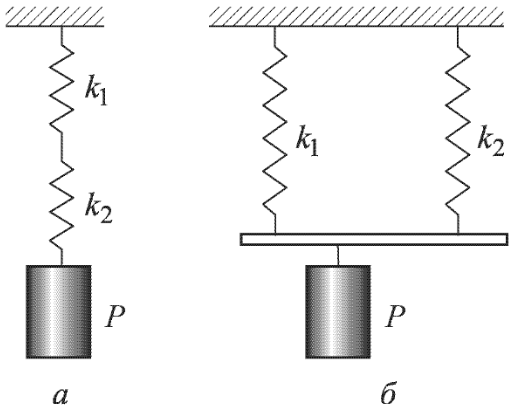
\includegraphics[width=0.5\textwidth]{2Springs.png}
\caption{}
\label{2Springs}
\end{figure}

\begin{ans}
1) $U_1/U_2 = k_2/k_1$; 2) $U_1/U_2 = k_1/k_2$.
\end{ans}
\end{ex}

\complexProblems

\begin{ex} %Сив197
Система состоит из двух шариков с массами $m$ и $M$, соединенных между собой невесомой пружиной с коэффициентом жесткости $k$ (рис. \ref{3BallsSpring}). Третий шарик с массой $m$, движущийся вдоль оси пружины со скоростью $v$, претерпевает упругое столкновение с шариком $m$, как указано на рис. \ref{3BallsSpring}. Считая шарики абсолютно жесткими, найти после столкновения: 1) кинетическую энергию $K$ движения системы как целого; 2) внутреннюю энергию системы $E_1$; 3) амплитуду колебаний одного шарика относительно другого $A$. До удара система покоилась, а пружина не была деформирована. Какие шарики могут рассматриваться как абсолютно жесткие?	

\begin{figure}[h]
\centering
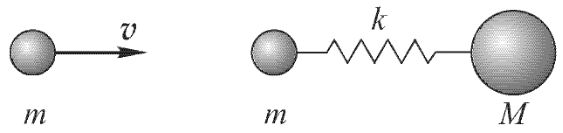
\includegraphics[width=0.5\textwidth]{3BallsSpring.png}
\caption{}
\label{3BallsSpring}
\end{figure}

\begin{ans}
1) $K=\frac{m^2v^2}{2(M+m)}$; 2) $E_1 = \frac{Mmv^2}{2(M+m)}$; 3) $A = v\sqrt{\frac{Mm}{k(M+m)}}$.
\end{ans}
\end{ex}

\begin{ex}  %Сив232
От поезда, идущего с постоянной скоростью, отрывается последний вагон, который проходит путь $l$ и останавливается. На каком расстоянии от вагона в момент его остановки будет находиться поезд, если тяга паровоза постоянна, а трение каждой части поезда не зависит от скорости и пропорционально ее весу? Масса поезда до момента отрыва вагона $M$, масса вагона $m$.
\begin{ans}
$x = Ml/(M-m)$.
\end{ans}
\end{ex}

\begin{ex} %Сив229
Два маятника в виде шариков разных масс $m_1$ и $m_2$ свободно подвешены на нитях разной длины $l_1$ и $l_2$ так, что шарики соприкасаются. Первый маятник отводят в плоскости нитей на угол $\alpha$ от первоначального положения и отпускают. Происходит центральный удар шариков. На какие углы $\alpha_1$ и $\alpha_2$ относительно отвесной линии отклонятся маятники после удара (углы считать малыми, удар считать упругим)?
\begin{ans}
$\alpha_1 =\frac{m_1-m_2}{m_1+m_2}\alpha$, $\alpha_2 =\frac{2m_1}{m_1+m_2}\alpha \sqrt{\frac{l_1}{l_2}}$.
\end{ans}
\end{ex}

\begin{ex} %Чертов2.69
Камешек скользит с наивысшей точки купола, имеющей форму полусферы. Какую дугу $\alpha$ опишет камушек, прежде чем оторвется от поверхности купола? Трением пренебречь.
\begin{ans}
$\alpha = \arccos(2/3)$.
\end{ans}
\end{ex}

\clearpage
\section{Динамика движения материальной точки по окружности}

\begin{ex} %Сив260
С какой начальной скоростью $v_0$ должен вылететь снаряд из орудия в горизонтальном направлении, чтобы двигаться вокруг Земли, не падая на нее? Каким ускорением будет обладать снаряд при этом (Радиус Земли $R = 6,4 \cdot 10^3$ км).
\begin{ans}
$v_0 = \sqrt{gR} \approx 8$ км/с.
\end{ans}
\end{ex}	

\begin{ex} %Сив273
Самолет делает «мертвую петлю» радиуса $R = 100$ м и движется по ней со скоростью $v = 280$ км/ч. С какой силой тело летчика массой в 80 кг будет давить на сиденье самолета в верхней и нижней точках петли?
\begin{ans}
$F_1 \approx 5,5$ кН; $F_2 \approx 4$ кН.
\end{ans}
\end{ex}	

\begin{ex}  %Сив264
На внутренней поверхности конической воронки с углом $2\alpha$ при вершине (рис. \ref{Conus}) на высоте $h$ от вершины находится малое тело. Коэффициент трения между телом и поверхностью воронки равен $\mu$. Найти минимальную угловую скорость вращения конуса вокруг вертикальной оси, при которой тело будет неподвижно в воронке.

\begin{figure}[h]
\centering
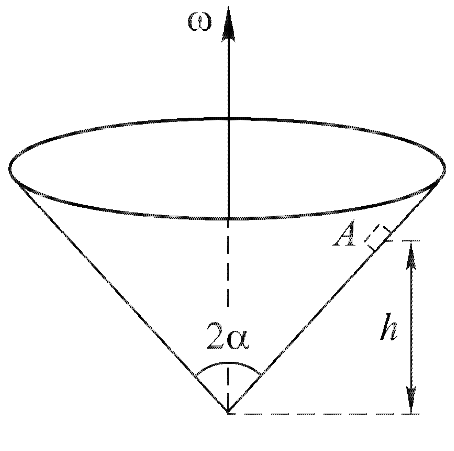
\includegraphics[width=0.3\textwidth]{Conus.png}
\caption{}
\label{Conus}
\end{figure}

\begin{ans}
$\omega^2 = \frac{g(\cos \alpha - \mu \sin \alpha)}{h \tg \alpha (\sin \alpha + \mu \cos \alpha)}$.
\end{ans}
\end{ex}	

\begin{ex} %Сив265
Велосипедист при повороте по кругу радиуса $R$ наклоняется внутрь закругления так, что угол между плоскостью велосипеда и землей равен $\alpha$. Найти скорость $v$ велосипедиста.
\begin{ans}
$v = \sqrt{Rg \ctg \alpha}$.
\end{ans}
\end{ex}	

\begin{ex} %Сив285
Металлическое кольцо, подвешенное на нити к оси центробежной машины, как указано на рис. \ref{RotationRing}, равномерно вращается с угловой скоростью $\omega$. Нить составляет угол $\alpha$ с осью. Найти расстояние от центра кольца до оси вращения.

\begin{figure}
\centering
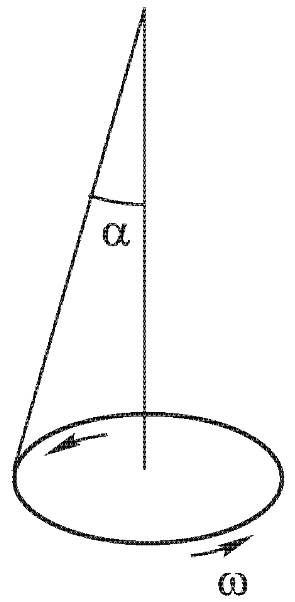
\includegraphics[width=0.25\textwidth]{RotationRing.png}
\caption{}
\label{RotationRing}
\end{figure}

\begin{ans}
$x = (g/\omega^2) \tg \alpha$.
\end{ans}
\end{ex}	


\begin{ex} %Сив283
Шарик массы $m$ подвешен на идеальной пружине жесткости $	k$ и начальной длины $l$ над центром платформы центробежной машины (рис. \ref{CentrafugalMashine}). Затем шарик начинает вращаться вместе с машиной с угловой скоростью $\omega$. Какой угол $\alpha$ образует при этом пружина с вертикалью?

\begin{figure}[h]
\centering
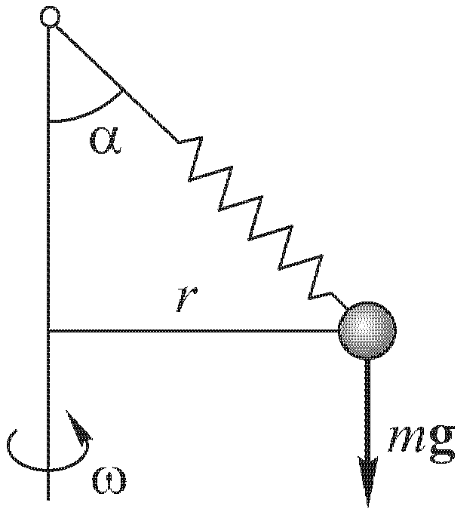
\includegraphics[width=0.3\textwidth]{CentrafugalMashine.png}
\caption{}
\label{CentrafugalMashine}
\end{figure}

\begin{ans}
$\alpha = 0$, если $\omega^2 < \frac{kg}{ml_0(g/l_0 + k/m)}$, иначе $\cos \alpha = g\frac{k-m\omega^2}{\omega^2kl_0}$ $\left( \omega < \sqrt{k/m} \right)$.
\end{ans}
\end{ex}	

\begin{ex} %Сив257
Найти силу $F$, с которой тележка массы $m$, движущаяся со скоростью $v$, давит на мост в одном из следующих случаев: 1) горизонтальный мост; 2) выпуклый мост (рис. \ref{Bridge}); 3) вогнутый мост. (Для случаев 2) и 3) силу $F$ определить для наивысшей и наинизшей точек моста).
\begin{ans}
1) $F=mg$; 2) $F=mg-\frac{mv^2}{R}$; 3) $F=mg+\frac{mv^2}{R}$.
\end{ans}
\end{ex}	

\begin{figure}[h]
\centering
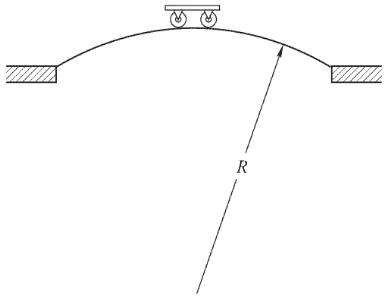
\includegraphics[width=0.5\textwidth]{Bridge.png}
\caption{}
\label{Bridge}
\end{figure}

\begin{ex} %Сив258
Тело движется прямолинейно с постоянной скоростью $v$ по горизонтальной поверхности стола, которая имеет закругленный край с постоянным радиусом закругления, равным $R$ (рис. \ref{Rounding}). Каково должно быть минимальное значение скорости $v_0$, чтобы тело, падая со стола, не касалось закругления?
\begin{ans}
$v_0 = \sqrt{gR}$.
\end{ans}
\end{ex}	

\begin{figure}[h]
\centering
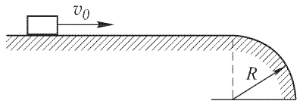
\includegraphics[width=0.5\textwidth]{Rounding.png}
\caption{}
\label{Rounding}
\end{figure}

\begin{ex} %Сив262
Тележка массы $m$ скатывается без трения по изогнутым рельсам, имеющим форму, изображенную на рис. \ref{DeathLoop}. 1) С какой минимальной высоты $h$ должна скатиться тележка для того, чтобы она не покинула рельсов по всей их длине? 2) Какие силы действуют на тележку в наивысшей точке $В$ петли? 3) Каково будет движение тележки, если она скатывается с высоты, меньшей $h$? При решении задачи считать колеса тележки малого размера и малой массы и их вращательного движения не рассматривать.
\begin{ans}
1) $h=5R/2$.
\end{ans}
\end{ex}	

\begin{figure}[h]
\centering
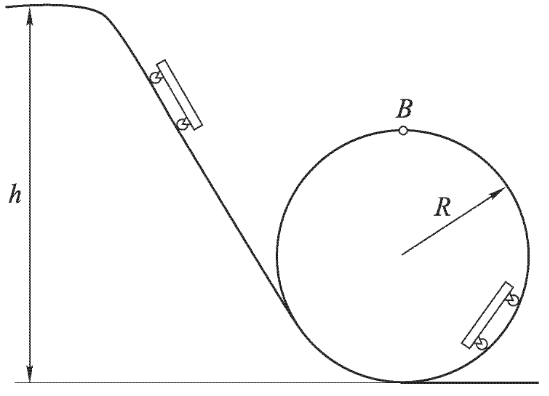
\includegraphics[width=0.5\textwidth]{DeathLoop.png}
\caption{}
\label{DeathLoop}
\end{figure}

\begin{ex}  %Сив263
Каков должен быть минимальный коэффициент трения скольжения к между шинами автомобиля и асфальтом, чтобы автомобиль мог пройти закругление с радиусом $R = 200$ м при скорости $v = 100$ км/ч?
\begin{ans}
$k=v^2/(gR) \approx 0,4$.
\end{ans}
\end{ex}	

\begin{ex}  %Сив267
Шарик радиуса $R$ висит на нити длины $l$ и касается вертикального цилиндра радиуса $r$, установленного на оси центробежной машины (рис. \ref{CentrafugalMashine2}). При какой угловой скорости и вращения центробежной машины шарик перестанет давить на стенку цилиндра?

\begin{figure}[h]
\centering
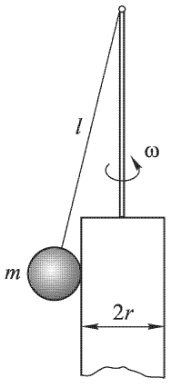
\includegraphics[width=0.2\textwidth]{CentrafugalMashine2.png}
\caption{}
\label{CentrafugalMashine2}
\end{figure}

\begin{ans}
$\omega^2 = g/\sqrt{(R+l)^2-(R+r)^2}$.
\end{ans}
\end{ex}	

\begin{ex} %Сив269
Шофер, едущий на автомобиле по горизонтальной площади в тумане, внезапно заметил недалеко впереди себя стену, перпендикулярную к направлению движения. Что выгоднее: затормозить или повернуть в сторону, чтобы предотвратить аварию?
\begin{ans}
Затормозить.
\end{ans}
\end{ex}	

\begin{ex} %Сив272 
При выполнении самолетом «мертвой петли», осуществленной впервые русским летчиком П. Н. Нестеровым, сила, действующая на крылья самолета, изменяется по сравнению с их нагрузкой при горизонтальном полете. Пусть самолет Нестерова массой в 3/4 т делает «мертвую петлю» радиуса $R = 235$ м и движется по ней со скоростью 120 км/ч. Найти максимальное значение нагрузки на крылья самолета. Указать, в каком месте траектории эта нагрузка будет максимальной.
\begin{ans}
$F = 14$ кН.
\end{ans}
\end{ex}	

\begin{ex} %Сив276
Груз массы $M$ может скользить без трения по стержню $a$, укрепленному перпендикулярно к оси вращающейся центробежной машины (рис. \ref{CentrafugalMashine3}). Ось машины вертикальна, и сквозь нее проходит нить, на которой висит груз массы $m$; нить перекинута через блок с и другой ее конец прикреплен к грузу массы $M$. Найти положение груза массы $M$ на стержне $a$ когда центробежная машина вращается с угловой скоростью $\omega$.

\begin{figure}[h]
\centering
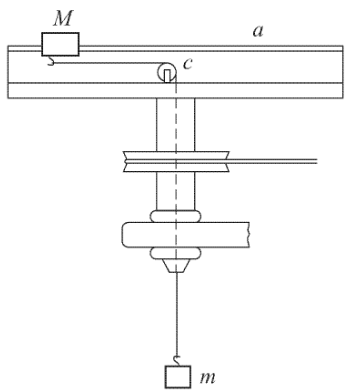
\includegraphics[width=0.4\textwidth]{CentrafugalMashine3.png}
\caption{}
\label{CentrafugalMashine3}
\end{figure}

\begin{ans}
$R = mg/(M\omega^2)$.
\end{ans}
\end{ex}	



\clearpage
\section{Основное уравнение вращательного движения}

\introProblems

\begin{ex} %Сив313
Найти ускорение грузов и натяжение нитей на машине, изображенной на рис. \ref{AtwoodInertia}, учитывая момент инерции $I$ вращающегося блока, при условии, что нить не скользит по блоку. Определить усилие в подвеске $A$, если масса блока равна $M$.
\begin{ans}
$a= \frac{m_2-m_1}{m_1+m_2+I/r^2}g$, $T_1 = \frac{2m_1m_2g + m_1gI/r^2}{m_1+m_2+I/r^2}$, $T_2 = \frac{2m_1m_2g + m_2gI/r^2}{m_1+m_2+I/r^2}$.
\end{ans}
\end{ex}	

\begin{ex}  %Сив314
Однородный цилиндр массы $M$ и радиуса $R$ (рис. \ref{CylinderInertia}) вращается без трения вокруг горизонтальной оси под действием веса груза $P$, прикрепленного к легкой нити, намотанной на цилиндр. Найти угол $\varphi$ поворота цилиндра в зависимости от времени, если при $t = 0$ $\varphi = 0$.
\begin{ans}
$\varphi = \frac{gt^2}{2R(1+Mg/2P)}$.
\end{ans}
\end{ex}	

\begin{figure}[h]
\centering
\begin{subfigure}{.33\textwidth}
  \centering
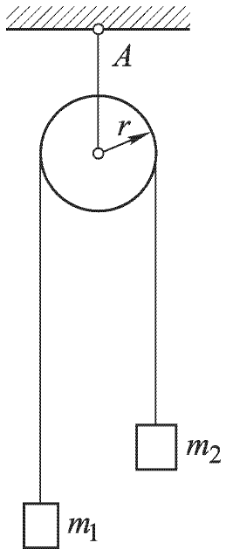
\includegraphics[width=0.6\textwidth]{AtwoodInertia.png}
\caption{}
\label{AtwoodInertia}
\end{subfigure}%
\begin{subfigure}{.33\textwidth}
  \centering
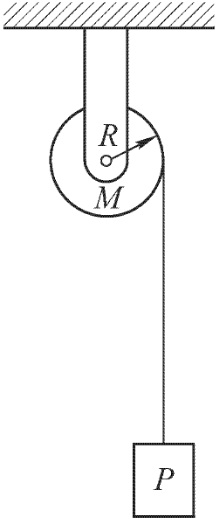
\includegraphics[width=0.6\textwidth]{CylinderInertia.png}
\caption{}
\label{CylinderInertia}
\end{subfigure}
\begin{subfigure}{.33\textwidth}
  \centering
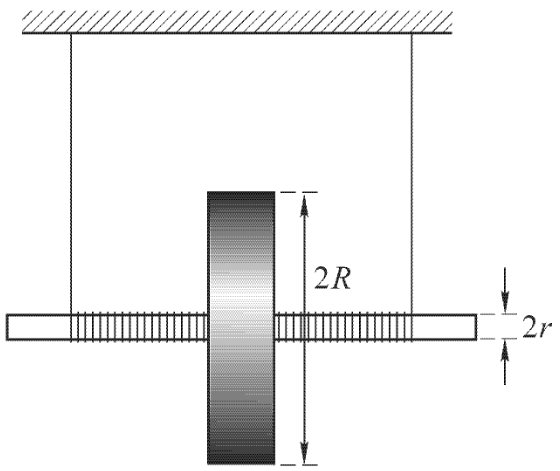
\includegraphics[width=1.2\textwidth]{MaxwellDisk.png}
\caption{}
\label{MaxwellDisk}
\end{subfigure}
\caption{}
\end{figure}

\begin{ex} %Сив319
Схема демонстрационного прибора (диск Максвелла) изображена на рис. \ref{MaxwellDisk}. На валик радиусом $r$ наглухо насажен сплошной диск радиуса $R$ и массы $M$. Валик и диск сделаны из одного материала, причем выступающие из диска части оси имеют массу $m$. К валику прикреплены нити одинаковой длины, при помощи которых прибор подвешивается к штативу. На валик симметрично наматываются нити в один ряд, благодаря чему диск поднимается, а затем предоставляют диску свободно опускаться. Найти ускорение, с которым опускается диск.
\begin{ans}
$a = \frac{2(M+m)r^2}{mr^2+MR^2+2(M+m)r^2}g$.
\end{ans}
\end{ex}	

\begin{ex} %Сив325
По наклонной плоскости, образующей угол $\alpha$ с горизонтом, скатывается без скольжения сплошной однородный диск. Найти линейное ускорение $a$ центра диска.
\begin{ans}
$a=2/3g\sin \alpha$.
\end{ans}
\end{ex}	

\begin{ex} %Сив333
На горизонтальной плоскости лежит катушка ниток. С каким ускорением $a$ будет двигаться ось катушки, если тянуть за нитку с силой $F$ (рис. \ref{Coil})? Каким образом	надо тянуть за нитку, чтобы катушка двигалась в сторону натянутой нитки? Катушка движется по поверхности стола без скольжения. Найти силу трения между катушкой и столом.
\begin{ans}
$a = \frac{F(R\cos \alpha - r)}{I + mR^2}$.
\end{ans}
\end{ex}	

\begin{figure}
\centering
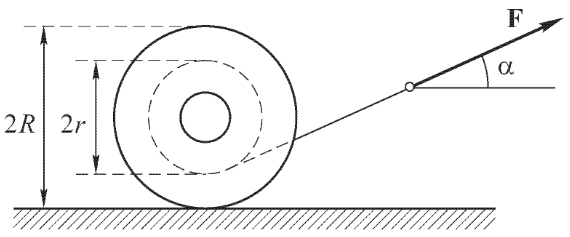
\includegraphics[width=0.5\textwidth]{Coil.png}
\caption{}
\label{Coil}
\end{figure}

\qualProblems

\begin{figure}[h]
\centering
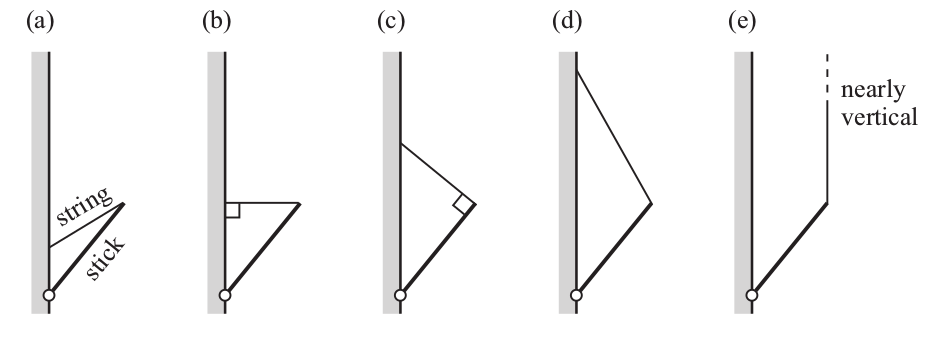
\includegraphics[width=0.75\textwidth]{tourqe.png}
\caption{}
\label{tourqe}
\end{figure}

\begin{ex}
Нижний конец стержня при помощи шарнира закреплен в стене, а его верхний конец прикреплен к стене при помощи невесомой нити различными способами, как показано на рисунке \ref{tourqe}. В каком случае сила натяжения нити будет минимальна?
\end{ex}	

\begin{ex}
Предложите экспериментальный способ определения массы бруска при помощи линейки и тела известной массы.
\end{ex}	

\begin{ex}
Известно, что диск и цилиндр имеют одинаковые массы и радиусы. Каково соотношение их моментов инерции относительно оси симметрии?
\end{ex}	

\begin{ex}
Четыре одинаковых небольших шарика соединили невесомыми стержнями таким образом, что получился квадрат. Во сколько раз момент инерции полученного квадрата относительно одной из сторон больше момента инерции относительно диагонали?
\end{ex}	

\begin{ex}
Какая форма и распределение массы должны быть у маховика, чтобы минимизировать массу и максимизировать момент инерции?
\end{ex}	

\begin{ex}
Цилиндрическое тело массы $m$ и радиуса $R$ имеет неоднородное распределение массы. Может ли масса быть распределенной таким образом, что момент инерции цилиндра относительно оси симметрии превышает $mR^2$? 
\end{ex}	

\begin{ex}
Выполняется ли закон сохранения энергии при скатывании цилиндра вдоль наклонной шероховатой плоскости без проскальзывания?
\end{ex}	

\begin{figure}[h]
\centering

\includegraphics[width=0.35\textwidth]{halfFrictionless.png}
\caption{}
\label{halfFrictionless}
\end{figure}

\begin{ex}
Шарик скатывается по полукруглой поверхности (рис. \ref{halfFrictionless}). Левая часть поверхности шероховатая, там шарик движется без проскальзывания. Правая часть поверхности - гладкая. Шарик начинает двигаться из состояния покоя с некоторой высоты $h$. Укажите верные утверждения:
\begin{itemize}
\item Из-за трения энергия не сохраняется, поэтому шарик поднимется справа на высоту меньшую $h$.
\item По закону сохранения энергии шарик поднимется справа на высоту меньшую $h$.
\item По закону сохранения энергии шарик поднимется справа на высоту равную $h$.
\item Вращение шарика позволит ему подняться справа на высоту большую $h$.
\end{itemize}
\end{ex}	

\simpleProblems

\begin{ex}
Определите момент инерции небольшого карандаша длиной 30 см и массой 50 г относительно оси вращения, перпендикулярной карандашу и проходящей через точку, отстоящую от середины карандаша на 1/6 часть его длины.
\end{ex}	

\begin{ex}
Сплошной диск массой 5 кг и радиусом 0,2 м вращается вокруг оси, перпендикулярной к диску и отстоящей от его центра на 10 см. Чему равен момент инерции диска относительно данной оси вращения?
\end{ex}	

\begin{ex}
В однородном диске массой $m = 1$ кг и радиусом $r = 30$ см вырезано круглое отверстие диаметром $d = 20$ см, центр которого находится на расстоянии $l = 15$ см от оси диска. Найти момент инерции $I$ полученного тела относительно оси, проходящей перпендикулярно плоскости диска через его центр.
\end{ex}	

\begin{ex}
Уравнение вращения шара массой 10 кг и радиусом 20 см вокруг оси, проходящей через его центр имеет вид: $\varphi = 1 + 4t^2 - t^3$. Все величины выражены в СИ. Вычислите вращающий момент, действующий на шар, через 2 с после начала вращения.
\end{ex}	

\begin{ex}
На горизонтальную ось насажены маховик и легкий шкив радиусом $R = 5$ см. На шкив намотан шнур, к которому привязан груз массой $m = 0.4$ кг. Опускаясь равноускорено, груз прошел путь $s = 1.8$ м за время $t = 3$ с. Определить момент инерции $I$ маховика. Массу шкива считать пренебрежимо малой.
\end{ex}	

\complexProblems

\begin{ex} %Сив316
На ступенчатый цилиндрический блок намотаны в противоположных направлениях две легкие нити, нагруженные массами $m_1$ и $m_2$ (рис. \ref{2BlocksInertia}). Найти угловое ускорение блока и натяжения $T_1$ и $T_2$ нитей, учитывая момент инерции $I$ блока.

\begin{figure}[h]
\centering
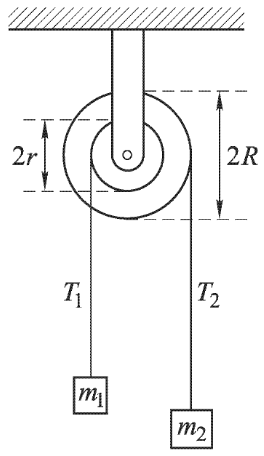
\includegraphics[width=0.25\textwidth]{2BlocksInertia.png}
\caption{}
\label{2BlocksInertia}
\end{figure}

\begin{ans}
$\varepsilon = \frac{m_2R - m_1r}{m_2R^2 + m_1r^2 + I}g$, $T_1 = m_1(g+r\varepsilon)$, $T_2 = m_2(g-R\varepsilon)$.
\end{ans}
\end{ex}	

\begin{ex} %Сив317
Модель ворота укреплена на одной чашке весов (рис. \ref{weighter}). На ворот с моментом инерции $I$ намотана нить с грузиком массы $m$. Весы уравновешены, когда ворот заторможен, и нить не разматывается. Насколько следует изменить вес гирь на другой чашке весов для того, чтобы восстановить равновесие, когда ворот вращается под действием опускающегося вниз грузика?
\begin{ans}
$\Delta m = m/(1+I/mr^2)$.
\end{ans}
\end{ex}	

\begin{figure}[h]
\centering
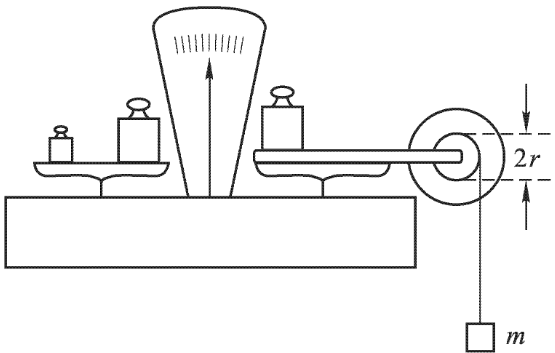
\includegraphics[width=0.4\textwidth]{weighter.png}
\caption{}
\label{weighter}
\end{figure}

\begin{ex} %Сив323
С каким ускорением $a$ будет опускаться катушка с массой $M$ и моментом инерции $I$ относительно оси симметрии, если она подвешена аналогично диску Максвелла (рис. \ref{coil2Threads}). На катушку намотаны еще две нити, к которым подвешен груз массы $m$. Определить натяжения нитей.

\begin{figure}
\centering
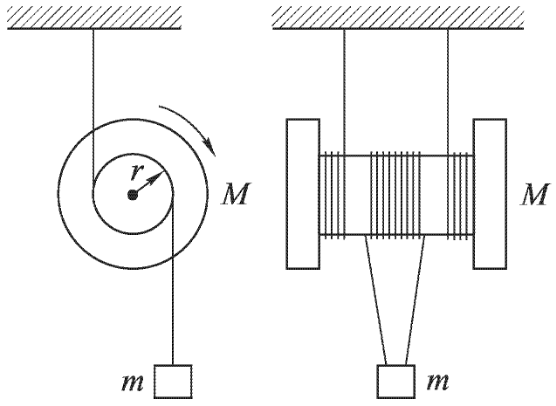
\includegraphics[width=0.4\textwidth]{coil2Threads.png}
\caption{}
\label{coil2Threads}
\end{figure}

\begin{ans}
$a = \frac{M+2m}{4m+M+I/r^2}g$, $T_1 = (2m+I/r^2)a - mg$, $T_2=m(g-2a)$.
\end{ans}
\end{ex}	

\begin{ex} %Сив326
Найти ускорение $a$ центра однородного шара, скатывающегося без скольжения по наклонной плоскости, образующей угол $\alpha$ с горизонтом. Чему равна сила трения сцепления шара и плоскости?
\begin{ans}
$a=5/7g\sin \alpha$.
\end{ans}
\end{ex}	

\begin{ex} %Сив328
По наклонной плоскости, составляющей с горизонтом угол $\alpha = 30^{\circ}$, скатывается без скольжения сплошной однородный цилиндр, масса которого равна 300 г. Найти величину силы трения цилиндра о плоскость.
\begin{ans}
$F = 1/3 mg \sin \alpha$.
\end{ans}
\end{ex}	

\begin{ex} %Сив329
Какова должна быть величина коэффициента трения $\mu$, чтобы однородный цилиндр скатывался без скольжения с наклонной плоскости, образующей угол $\alpha$ с горизонтом?
\begin{ans}
$\mu > 1/3 \tg \alpha$.
\end{ans}
\end{ex}	

\begin{ex} %Сив332
К тележке, стоящей на горизонтальной плоскости, привязана нить, перекинутая через блок, укрепленный у края стола; к концу нити прикреплен груз массы $m_3$ = 500 г. Определить ускорение тележки $a$, если известно, что масса платформы тележки $m_1$ = 1,4 кг, масса каждого колеса $m_2$ = 400 г и колеса представляют собой сплошные диски. Колеса катятся по поверхности стола без скольжения, а трение качения отсутствует.
\begin{ans}
$a = m_3g/(m_1 + 6m_2 +m_3)$.
\end{ans}
\end{ex}	

\clearpage
\section{Законы сохранения момента импульса и энергии}

\introProblems

\begin{ex} %Сив337
Однородный тонкий тяжелый стержень длины $l$ висит на горизонтальной оси, проходящей через один из его концов. Какую начальную угловую скорость и надо сообщить стержню, чтобы он повернулся на $90^{\circ}$?
\begin{ans}
$\omega = \sqrt{3g/l}$.
\end{ans}
\end{ex}	

\begin{ex} %Сив340
На краю свободно вращающегося достаточно большого горизонтального диска, имеющего радиус $R$ и момент инерции $I$, стоит человек массы $m$. Диск совершает $\nu$ об/мин. Как изменится скорость вращения диска, если человек перейдет от края диска к центру? Как изменится при этом энергия системы? Размерами человека по сравнению с радиусом диска можно пренебречь.
\begin{ans}
Скорость вращения возрастет в $(1+mR^2/I)$ раз.
\end{ans}
\end{ex}	

\begin{ex} %Сив341
На покоящемся однородном горизонтальном диске массы $M$ и радиуса $R$ находится человек массы $m$. Диск может вращаться без трения вокруг вертикальной оси, проходящей через его центр. В некоторый момент человек начал двигаться. С какой угловой скоростью вращается диск, когда человек идет по окружности радиуса $r$, концентричной диску, со скоростью $v$ относительно диска?
\begin{ans}
$\omega = mrv/(0,5MR^2 + mr^2)$.
\end{ans}
\end{ex}	

\begin{figure}[h]
\centering
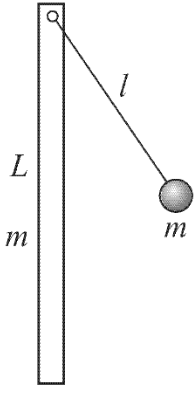
\includegraphics[width=0.17\textwidth]{rodBall.png}
\caption{}
\label{rodBall}
\end{figure}

\begin{ex} %Сив359
Тонкий стержень массы $m$ и длины $L$ (рис. \ref{rodBall}) подвешен за один конец и может вращаться без трения вокруг горизонтальной оси. К той же оси подвешен на нити длины $l$ шарик такой же массы $m$. Шарик отклоняется на некоторый угол и отпускается. При какой длине нити шарик после удара о стержень остановится? Считать удар абсолютно упругим.
\begin{ans}
$l = L/\sqrt{3}$.
\end{ans}
\end{ex}	

\begin{ex}  %Сив359
Каким участком сабли следует рубить лозу, чтобы рука не чувствовала удара? Саблю считать однородной пластинкой.
\begin{ans}
Лозу следует рубить участком сабли, отстоящим на $2/3$ длины от ручки сабли.
\end{ans}
\end{ex}	

\qualProblems

\begin{ex}
Который из следующих объектов обладает наибольшим моментом импульса относительно точки $P$ (рис. \ref{AngularMomentum})? Стрелки указывают на направления вращения и на скорости центров масс дисков, на всех рисунках эти величины имеют одинаковые значения (стрелки равной длины).
\end{ex}	

\begin{figure}[h]
\centering
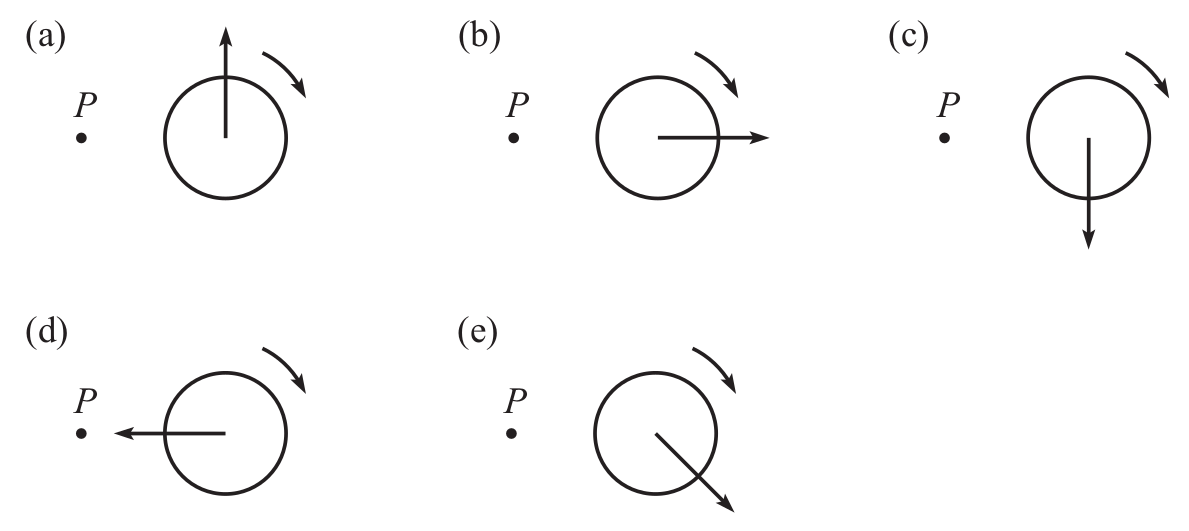
\includegraphics[width=0.8\textwidth]{AngularMomentum.png}
\caption{}
\label{AngularMomentum}
\end{figure}

\begin{ex}
Обладает ли количеством движения (импульсом) однородный диск, вращающийся вокруг своей оси? Ось диска неподвижна.
\end{ex}	

\begin{ex}
Мотоциклист совершает прыжок через колонну автомобилей. Сразу после взлета он заметил, что мотоцикл наклонился немного назад. Если этот наклон сохранится, что у него возникнут проблемы при приземлении, т.к. в тот момент мотоцикл должен быть наклонен немного вперед. Как нужно поступить мотоциклисту, чтобы исправить ситуацию:
\begin{itemize}
\item наклониться вперед;
\item наклониться назад;
\item нажать на газ;
\item нажать на тормоз;
\end{itemize}
\end{ex}	

\begin{ex}
Балерина на льду — вот прекрасный пример, иллюстрирующий закон сохранения момента  импульса. Когда балерина прижимает руки к телу, ее вращение ускоряется именно благодаря сохранению момента импульса (внешние моменты сил при этом отсутствуют). Это, конечно, так, но как объяснить такое явление с точки зрения сил, действующих на балерину,— ведь нам гораздо легче оперировать с силами, чем с моментами импульса. Какая же сила ускоряет вращение балерины?
\end{ex}	


\simpleProblems

\begin{ex}
Тонкий прямой стержень длиной $l = 1$ м прикреплен к горизонтальной оси, проходящей через его конец. Стержень отклонили на угол $\varphi = 60^{\circ}$ от положения равновесия и отпустили. Определить линейную скорость $v$ нижнего конца стержня в момент прохождения через положение равновесия.
\end{ex}	

\begin{ex} %Чертов3.31
Человек стоит на скамье Жуковского и ловит рукой мяч массой $m = 0,4$ кг, летящий в горизонтальном направлении со скоростью $v = 20$ см/с. Траектория мяча проходит на расстоянии $r=0,8$ м от вертикальной оси вращения скамьи. С какой угловой скорость начнет вращаться скамья Жуковского с человеком, поймавшим мяч, если суммарный момент инерции человека и скамьи равен 6 кг$\cdot$м\textsuperscript{2}?
\begin{ans}
$\omega = mvr/(I+mr^2) = 1$ рад/с.
\end{ans}
\end{ex}	

\begin{ex} %Чертов3.45
Кинетическая энергия вращающегося маховика равна 1 кДж. Под действием постоянного тормозящего момента маховик начал вращаться равнозамедленно и, сделав 80 оборотов, остановился. Определите момент силы торможения.
\begin{ans}
$M = E / (2 \pi N) = 2$ Нм.
\end{ans}
\end{ex}	

\begin{ex}
Шарик массой $m = 100$ г, привязанный к концу нити длиной $l_1 = 1$ м, вращается, опираясь на горизонтальную плоскость, с частотой $\nu_1 = 1$ с\textsuperscript{-1}. Нить укорачивается и шарик приближается к оси вращения до расстояния $l_2 = 0.5$ м. С какой частотой $\nu_2$ будет при этом вращаться шарик? Какую работу $A$ совершит внешняя сила, укорачивая нить? Трением шарика о плоскость пренебречь.
\end{ex}	

\begin{ex} %Сив342
Экспериментатор стоит на специальной табуретке и держит в руках вертикальную ось свободно вращающегося колеса, имеющего момент инерции $I_1$ относительно этой оси $AA$ (рис. \ref{hyroscop}). Колесо вращается в горизонтальной плоскости с угловой скоростью $\omega$. Табуретка устроена так, что она может свободно вращаться вокруг вертикальной оси, т. е. представляет собой так называемую скамью Жуковского. Момент инерции табуретки и экспериментатора вокруг вертикальной оси равен $I_2$. Ось колеса и ось табуретки лежат на одной прямой. На какую величину $\Delta E$ изменится кинетическая энергия всей системы табуретки и колеса, если экспериментатор повернет ось колеса на $180^{\circ}$, на $90^{\circ}$?

\begin{figure}[h]
\centering
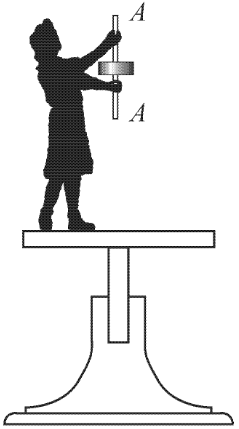
\includegraphics[width=0.25\textwidth]{hyroscop.png}
\caption{}
\label{hyroscop}
\end{figure}

\begin{ans}
1) $\Delta E = 2I_1^2\omega^2/I_2$; 2) $\Delta E = I_1^2\omega^2/2I_2$.
\end{ans}
\end{ex}	

\complexProblems

\begin{ex} %Сив357
Вертикально висящая однородная доска длины $L = 1,5$ м и массы $M = 10$ кг может вращаться вокруг горизонтальной оси, проходящей через ее верхний конец. В нижний конец доски ударяет пуля, летящая горизонтально с начальной скоростью $v_0$ = 600 м/с. Пуля пробивает доску и летит далее со скоростью $v$. Определить скорость $v$, если после выстрела доска стала колебаться с угловой амплитудой $\alpha  = 0,1$ рад. Масса пули $m = 10$ г.
\begin{ans}
$v = v_0 -M/m \sqrt{2gL/3} \sin \alpha /2 = 444$ м/с.
\end{ans}
\end{ex}	


\begin{ex} %Сив343
Монета массы $m$ и радиуса $r$, вращаясь в горизонтальной плоскости вокруг своей геометрической оси с угловой скоростью $\omega$ вертикально падает на горизонтальный диск и «прилипает» к нему. В результате диск приходит во вращение вокруг своей оси. Возникающий при этом момент сил трения в оси диска постоянен и равен $M_0$. Через какое время вращение диска прекратится? Сколько оборотов $N$ сделает диск до полной остановки? Момент инерции диска относительно его геометрической оси $I_0$. Расстояние между осями диска и монеты равно $d$.
\begin{ans}
$t = m\omega r^2 / 2M_0$, $N = M_0t^2/2I$, $I = I_0 + m(d^2 + r^2/2)$.
\end{ans}
\end{ex}	

\begin{ex} %Сив345
На горизонтальный диск, вращающийся вокруг геометрической оси с угловой скоростью $\omega_1$, падает другой диск, вращающийся вокруг той же оси с угловой скоростью $\omega_2$. Моменты инерции дисков относительно указанной оси равны соответственно $I_1$ и $I_2$. Оба диска при ударе сцепляются друг с другом (при помощи острых шипов на их поверхностях). На сколько изменится общая кинетическая энергия вращения системы после падения второго диска? Чем объясняется изменение энергии Геометрические оси обоих дисков являются продолжением одна другой.
\begin{ans}
$\Delta E = I_1 I_2 (\omega_1 - \omega_2)^2/ 2(I_1 + I_2)$.
\end{ans}
\end{ex}	

\begin{figure}[h]
\centering
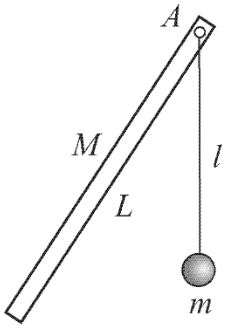
\includegraphics[width=0.22\textwidth]{collisionRod.png}
\caption{}
\label{collisionRod}
\end{figure}

\begin{ex} %Сив358
В общей точке подвеса $A$ (рис. \ref{collisionRod}) подвешены шарик на нити длины $l$ и однородный стержень длины $L$, отклоненный в сторону на некоторый угол. При возвращении стержня в положение равновесия происходит упругий удар. При каком соотношении между массами стержня $M$ и шарика $m$ шарик и точка удара стержня будут двигаться после удара с равными скоростями
в противоположных направлениях? При каком соотношении между
массами $M$ и $m$ описанный процесс невозможен?
\begin{ans}
$ML^2 = ml^2$, при $M \leq m$.
\end{ans}
\end{ex}	

\begin{ex} %Сив348
Однородный диск $A$ массы $M_1$ и радиуса $r_1$ (рис. \ref{2Disks}) раскручен до угловой скорости $\omega_0$ и приведен в контакт с диском $B$, ось вращения которого перпендикулярна к оси диска $A$. Масса диска $B$ равна $M_2$, а расстояние между точкой соприкосновения и осью диска $A$ равно $a$. Найти установившиеся угловые скорости дисков $\omega_1$ и $\omega_2$ и потерю энергии в процессе установления. Трением в осях, а также трением качения пренебречь.

\begin{figure}[h]
\centering
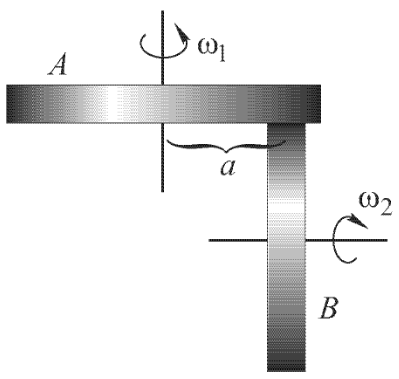
\includegraphics[width=0.4\textwidth]{2Disks.png}
\caption{}
\label{2Disks}
\end{figure}

\begin{ans}
$\omega_1 = \frac{M_1r_1^2\omega_0}{M_1r_1^2 + M_2a^2}$, $\omega_2 = \frac{M_1r_1^2 a \omega_0}{(M_1r_1^2 + M_2a^2)r_2}$, $\Delta E = \frac{M_1 M_2r_1^2a^2\omega_0^2}{4(M_1r_1^2 + M_2a^2)}$.
\end{ans}
\end{ex}	

\begin{ex} %Сив354

\begin{figure}[h]
\centering
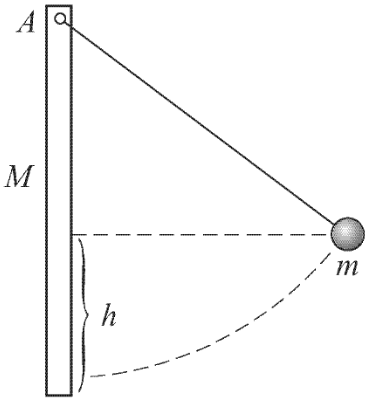
\includegraphics[width=0.3\textwidth]{rodOscil.png}
\caption{}
\label{rodOscil}
\end{figure}

Математический маятник массы $m$ и стержень массы $M$ (рис. \ref{rodOscil}) подвешены к одной и той же точке $A$, вокруг которой они могут свободно колебаться. Длина нити маятника равна длине стержня. Шарик маятника отклоняют в сторону, так что он приподнимается на высоту $h$ относительно своего нижнего положения. Затем шарик отпускают, и он сталкивается неупруго со стержнем. Как будут двигаться шарик и нижний конец стержня после удара и на какие высоты они поднимутся? Как изменится ответ задачи, если первоначально нижний конец стержня был поднят на высоту $h$?
\begin{ans}
После удара шарик и стержень будут подниматься как единое тело на высоту $h = \frac{6m^2}{(M+2m)(M+3m)}H$.
\end{ans}
\end{ex}	

\begin{ex} %Сив344
Сплошной однородный короткий цилиндр радиуса $r$, вращающийся вокруг своей геометрической оси с частотой $\nu$ об/с, ставят в вертикальном положении на горизонтальную поверхность. Сколько оборотов $N$ сделает цилиндр, прежде чем вращение его полностью прекратится? Коэффициент трения скольжения между основанием цилиндра и поверхностью, на которую он поставлен, не зависит от скорости вращения и равен $\mu$.
\begin{ans}
$N = 2\pi r n^2/(4 \mu g)$.
\end{ans}
\end{ex}	

\clearpage
\section{Вращательное движение твердого тела}

\introProblems

\begin{ex} %Сив362
Стержень массы $M$ и длины $l$, который может свободно вращаться вокруг неподвижной горизонтальной оси, проходящей через один из его концов, под действием силы тяжести переходит из горизонтального положения в вертикальное (рис. \ref{rodHitMass}). Проходя через вертикальное положение, нижний конец стержня упруго ударяет о малое тело массы $m$, лежащее на гладком горизонтальном столе. Определить скорость тела $m$ после удара.
\begin{ans}
$v = 2M\sqrt{3gl}/(M+3m)$.
\end{ans}
\end{ex}	

\begin{figure}[h]
\centering
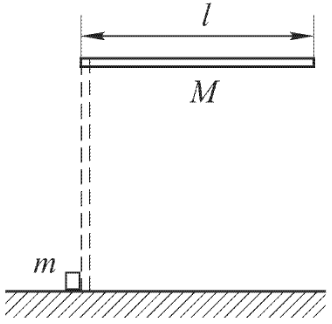
\includegraphics[width=0.35\textwidth]{rodHitMass.png}
\caption{}
\label{rodHitMass}
\end{figure}

\begin{ex} %Сив373
На двух параллельных горизонтальных брусьях лежит сплошной цилиндр радиуса $R$ и массы $m$, на который намотана веревка. К опущенному вниз концу веревки приложена вертикальная сила $F$, равная половине веса цилиндра (рис. \ref{rollingCylinder2}). Найти горизонтальное ускорение цилиндра и минимальное значение коэффициента трения между цилиндром и брусьями, при котором будет происходить качение без скольжения. Ось цилиндра перпендикулярна к брусьям, центр его масс и сила $F$ лежат в вертикальной плоскости, проходящей посередине между брусьями.
\begin{ans}
$a = g/3$, при $\mu \leq 2/9$.
\end{ans}
\end{ex}	

\begin{figure}[h]
\centering
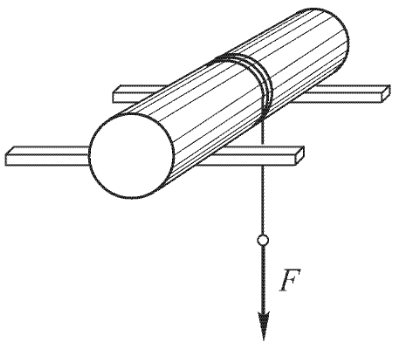
\includegraphics[width=0.4\textwidth]{rollingCylinder2.png}
\caption{}
\label{rollingCylinder2}
\end{figure}

\begin{ex} %Сив393
Сплошной однородный шар радиуса $r$, вращающийся вокруг горизонтального диаметра с угловой скоростью $\omega_0$, ставится на горизонтальную плоскость без сообщения ему поступательного движения. Учитывая трение скольжения, но пренебрегая трением качения, найти линейную скорость $v$ центра шара, когда его движение перейдет в чистое качение. Определить потерю кинетической энергии на трение.
\begin{ans}
$v = 2/7r \omega_0$, $\Delta E = 1/7 mr^2 \omega_0^2$.
\end{ans}
\end{ex}	

\qualProblems

\begin{ex}
Может ли одна сила, приложенная к твердому телу, изменить его поступательное движение и вращательное движение?
\end{ex}	

\begin{ex}
Когда канатоходец идет по канату, он расставляет руки в стороны для того чтобы сохранять равновесие. Объясните этот механизм с точки зрения основного уравнения вращательного движения твердого тела.
\end{ex}	

\simpleProblems

\begin{ex} %Сив366
Вертикальный столб высотой $l$ подпиливается у основания и падает на землю, поворачиваясь вокруг нижнего основания. Определить линейную скорость его верхнего конца в момент удара о землю. Какая точка столба будет в этот момент иметь ту же скорость, какую имело бы тело, падая с той, же высоты, как и данная точка?
\begin{ans}
$v = \sqrt{3gl}$, $x = 2/3l$.
\end{ans}
\end{ex}	

\begin{ex} %Сив369
Гимнаст на перекладине выполняет большой оборот из стойки на руках, т.е. вращается, не сгибаясь, вокруг перекладины под действием собственного веса. Оценить приближенно наибольшую нагрузку $F$ на его руки, пренебрегая трением ладоней о перекладину.
\begin{ans}
Если при оценке человека моделировать однородным стержнем, получим $F = 4mg$.
\end{ans}
\end{ex}	

\begin{ex} %Сив379
К шкиву креста Обербека (рис. \ref{oberbek}) прикреплена нить, к которой подвешен груз массы $M = 1$ кг. Груз опускается с высоты $h = 1$ м до нижнего положения, а затем начинает подниматься вверх. В это время происходит «рывок», т.е. увеличение натяжения нити. Найти натяжение нити $T$ при опускании или поднятии груза, а также оценить приближенно натяжение во время рывка $T_1$. Радиус шкива $r = З$ см. На кресте укреплены четыре груза с массой $m = 250$ г каждый на расстоянии $R = 30$ см от его оси. Моментом инерции самого креста и шкива пренебречь по сравнению с моментом инерции грузов. Растяжение нити во время рывка не учитывать.
\begin{ans}
$T = Mg/(1 + Mr^2/(4mR^2))$, $T_1 = Mg + MhrT/(\pi m R^2)$.
\end{ans}
\end{ex}	

\begin{figure}[h]
\centering
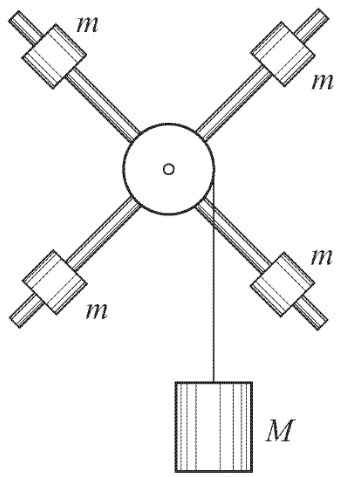
\includegraphics[width=0.3\textwidth]{oberbek.png}
\caption{}
\label{oberbek}
\end{figure}

\complexProblems

\begin{ex} %Сив374
К концу веревки, намотанной на цилиндр привязан груз массы $M$. Веревка переброшена через блок, как показано на рис. \ref{slipCylinder}. Определить ускорение груза $M$. Выяснить условия, при которых качение цилиндра будет происходить со скольжением. Весом веревки и блока, а также силами трения на оси блока можно пренебречь. Считать, что во всех случаях движение цилиндра будет плоскопараллельным.
\begin{ans}
$a = g/(1+3m/8M)$, при отсутствии скольжения $\mu /leq (8+3m/M)^{-1}$; $a = g(1 - \mu m/3M)/(1+m/3M)$, при скольжении $\mu < (8+3m/M)^{-1}$.
\end{ans}
\end{ex}	

\begin{figure}[h]
\centering
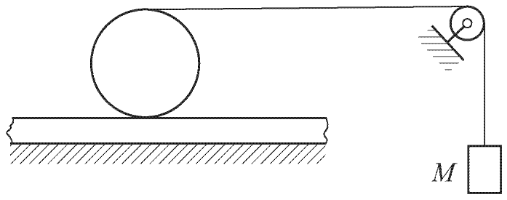
\includegraphics[width=0.5\textwidth]{slipCylinder.png}
\caption{}
\label{slipCylinder}
\end{figure}

\begin{ex} %Сив376
Два катка, связанные штангой $S$, скатываются без скольжения с наклонной плоскости, образующей угол в $30^{\circ}$ с горизонтом (рис. \ref{2rolling}). Катки имеют одинаковые массы $m = 5$ кг и одинаковые радиусы $R = 5$ см, момент инерции первого $I_1 = 80$ кгсм\textsuperscript{2}, второго $I_2 = 40$ кгсм\textsuperscript{2}. Массами рам катков и штанги можно пренебречь. Подсчитать угловое ускорение, с которым катки скатываются без скольжения с наклонной плоскости. Определить силу, передаваемую штангой, если каток с большим моментом инерции движется впереди, и наоборот.
\begin{ans}
$\varepsilon = \frac{2Rg \sin \alpha}{(I_1 + I_2)/m + 2R^2} \approx 66$ c\textsuperscript{-2}.
\end{ans}
\end{ex}	

\begin{figure}[h]
\centering
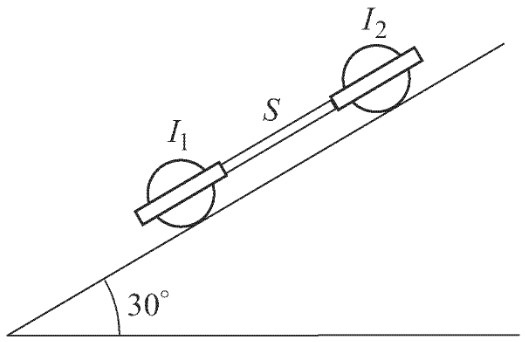
\includegraphics[width=0.5\textwidth]{2rolling.png}
\caption{}
\label{2rolling}
\end{figure}

\begin{ex} %Сив391
Сплошной цилиндр, ось которого горизонтальна, движется без вращения по гладкой горизонтальной плоскости в направлении, перпендикулярном к его оси. В некоторый момент цилиндр достигает границы, где поверхность становится шероховатой и возникает постоянная (не зависящая от скорости) сила трения скольжения, а трение качения отсутствует. Каково будет движение цилиндра после перехода границы? Как распределится кинетическая энергия поступательного движения цилиндра?
\begin{ans}
Движение после перехода границы будет сначала равнозамедленное, а затем с постоянной скоростью; 1/3 энергии превратится в тепло, 2/9 — во вращательную энергию и 4/9 останется в виде энергии поступательного движения.
\end{ans}
\end{ex}	

\begin{ex} %Сив383

\begin{figure}[h]
\centering
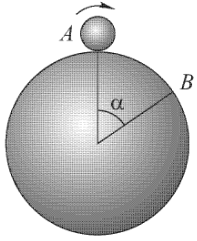
\includegraphics[width=0.25\textwidth]{ballSphere.png}
\caption{}
\label{ballSphere}
\end{figure}

Шарик радиуса $r$ скатывается без начальной скорости и без скольжения по поверхности сферы из самого верхнего положения $A$ (рис. \ref{ballSphere}). Определить положение точки $B$, в которой он оторвется от сферы и начнет свободно двигаться под действием силы тяжести.
\begin{ans}
$\cos \alpha = 10/17$.
\end{ans}
\end{ex}	

\clearpage
\section{Механические колебания}

\begin{ex} %Сив557
Построить графики зависимости от времени смещения, скорости и ускорения при простом гармоническом колебании. Построить графики зависимости скорости и ускорения от смещения. Найти соотношения между амплитудами смещения, скорости и ускорения.
\begin{ans}
$v_m = \omega A$, $a_m = \omega^2 A$.
\end{ans}
\end{ex}	

\begin{figure}[h]
\centering
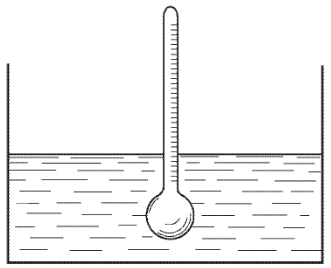
\includegraphics[width=0.35\textwidth]{areometr.png}
\caption{}
\label{areometr}
\end{figure}

\begin{ex} %Сив560
Ареометр с цилиндрической трубкой диаметра $D$ (рис. \ref{areometr}), плавающий в жидкости плотности $\rho$, получает небольшой вертикальный толчок. Найти период колебаний $T$ ареометра, если масса его $m$ известна. Движение жидкости и ее сопротивление движению ареометра не учитывать.
\begin{ans}
$T = 4 \sqrt{\pi m / g \rho D^2}$.
\end{ans}
\end{ex}	

\begin{figure}[h]
\centering
\includegraphics[width=0.5\textwidth]{oscilString.png}
\caption{}
\label{oscilString}
\end{figure}

\begin{ex} %Сив572
Найти период свободных малых колебаний грузика массы $m$, укрепленного на середине тонкой струны длины $L$ (рис. \ref{oscilString}). Массой струны можно пренебречь; натяжение струны постоянно и равно $P$.
\begin{ans}
$T = \pi \sqrt{m L /P}$.
\end{ans}
\end{ex}	

\begin{ex} %Сив580
Горизонтальная мембрана совершает синусоидальные колебания с круговой частотой $\omega$ и и амплитудой $A$. На мембране лежит маленький грузик. При каком условии грузик будет колебаться вместе с мембраной и при каком он начнет подскакивать?
\begin{ans}
При $\omega^2 A > g$ грузик будет подскакивать.
\end{ans}
\end{ex}	

\begin{figure}[h]
\centering
\includegraphics[width=0.25\textwidth]{fallingOnPlate.png}
\caption{}
\label{fallingOnPlate}
\end{figure}

\begin{ex} %Сив582
На чашку весов, подвешенную на пружине, падает с высоты $h$ груз массы $m$ и остается на чашке (рис. \ref{fallingOnPlate}), не подпрыгивая относительно нее. Чашка начинает колебаться. Коэффициент жесткости пружины $k$. Определить амплитуду $A$ колебаний (массой чашки и пружины по сравнению с массой груза можно пренебречь).
\begin{ans}
$A = \frac{mg}{k}\sqrt{ 1 + \frac{2hk}{mg}}$.
\end{ans}
\end{ex}	

\begin{ex} %Сив558
Найти выражения для потенциальной, кинетической и полной энергии материальной точки массы $m$, совершающей гармоническое колебание по закону $A \cos \omega t$.
\begin{ans}
$E_1 = m A^2 \omega^2 (1 - \cos 2 \omega t)/4$, $E_2 = m A^2 \omega^2 (1 + \cos 2 \omega t)/4$, $E = m A^2 \omega^2 /2$.
\end{ans}
\end{ex}	

\begin{ex} %Сив565
Представьте себе шахту, пронизывающую земной шар по одному из его диаметров. Найти закон движения тела, упавшего в эту шахту, учитывая изменения значения ускорения свободного падения внутри Земли. Трение о стенки шахты и сопротивление воздуха не учитывать.
\begin{ans}
Гармоническое колебание с периодом $T = 2 \pi \sqrt{R_0 / g_0}$, где $R_0$ -- радиус земного шара, $g_0$ -- ускорение свободного падения на поверхности Земли.
\end{ans}
\end{ex}	

\begin{figure}[h]
\centering
\includegraphics[width=0.25\textwidth]{removePlate.png}
\caption{}
\label{removePlate}
\end{figure}

\begin{ex} %Сив575
К пружине, один конец которой закреплен, подвешен груз $P$ массы $m$, лежащий на подставке так, что пружина не растянута (рис. \ref{removePlate}). Без толчка подставка убирается. Найти движение груза и максимальное натяжение пружины. Коэффициент жесткости пружины $k$.
\begin{ans}
$x = mg/k(1-\cos \sqrt{g/m} t)$.
\end{ans}
\end{ex}	

\begin{ex} %Сив577
На доске лежит груз весом $Р = 10$ Н. Доска совершает гармоническое колебание в вертикальном направлении с периодом $T = 1/2$ с и амплитудой $A = 2$ см. Определить величину силы давления $F$ груза на доску. С какой амплитудой А должна колебаться доска, чтобы груз начал отскакивать от доски?
\begin{ans}
$A \approx 6,2$ см.
\end{ans}
\end{ex}	

\begin{ex} %Сив581
Доска совершает гармоническое колебание в горизонтальном направлении с периодом $T = 5$ с. Лежащее на ней тело начинает скользить, когда амплитуда колебания достигает величины $A = 0,6$ м. Каков коэффициент трения покоя к между грузом и доской?
\begin{ans}
$\mu = 4 \pi^2 A / (gT^2) = 0,1$.
\end{ans}
\end{ex}	

\clearpage
\section{Колебания физического маятника}

\introProblems

\begin{ex} %Сив599
В какой точке следует подвесить однородный стержень длины  $l$, чтобы частота его колебаний, как физического маятника, была максимальна? Чему равна эта частота?
\begin{ans}
$x = l/(2\sqrt{3})$, $\omega^2 = g\sqrt{3} / l$.
\end{ans}
\end{ex}	

\begin{ex} %Сив602
На горизонтальной плоскости находится цилиндр с моментом инерции $I$ (относительно продольной геометрической оси), массой $m$ и радиусом $r$. К оси цилиндра прикреплены две одинаковые горизонтально расположенные спиральные пружины, другие концы которых закреплены в стене (рис. \ref{rollOscil}, вид сверху). Коэффициент жесткости каждой пружины равен $k$; пружины могут работать как на растяжение, так и на сжатие. Найти период малых колебаний цилиндра, которые возникнут, если вывести его из положения равновесия и дать возможность кататься без скольжения по горизонтальной плоскости.
\begin{ans}
$T =  \pi\sqrt{3m/k}$.
\end{ans}
\end{ex}	

\begin{figure}[h]
\centering
\includegraphics[width=0.4\textwidth]{rollOscil.png}
\caption{}
\label{rollOscil}
\end{figure}

\begin{ex} %Сив607
Найти период малых колебаний физического маятника массы $m$, к центру масс $C$ которого прикреплена горизонтальная спиральная пружина с коэффициентом жесткости $k$. Другой конец пружины закреплен в неподвижной стенке (рис. \ref{physPend}). Момент инерции маятника относительно точки подвеса равен $I$, расстояние между точкой подвеса и центром масс маятника равно $a$. В положении равновесия пружина не деформирована.
\begin{ans}
$T = 2 \pi \sqrt{I/(mga + ka^2)}$.
\end{ans}
\end{ex}	

\begin{figure}[h]
\centering
\includegraphics[width=0.3\textwidth]{physPend.png}
\caption{}
\label{physPend}
\end{figure}

\begin{ex} %Сив608
Колебательная система состоит из однородного стержня длины $l$ и массы $m$, который может вращаться вокруг горизонтальной оси $O$, проходящей через его конец и перпендикулярной к продольной оси стержня (рис. \ref{springRodOsc}). Другой конец стержня подвешен на пружине с коэффициентом жесткости $k$. Расстояние между серединой стержня и осью вращения $CO = a$. Момент инерции стержня относительно оси $O$ равен $I$. Найти удлинение пружины $x_0$ (по сравнению с ее длиной в недеформированном состоянии) в положении равновесия, если в этом $O$ положении стержень горизонтален. Определить также период малых колебаний стержня около положения равновесия.
\begin{ans}
$x_0 = mga/kl$, $T = 2 \pi \sqrt{I/kl^2}$.
\end{ans}
\end{ex}	

\begin{figure}[h]
\centering
\includegraphics[width=0.3\textwidth]{springRodOsc.png}
\caption{}
\label{springRodOsc}
\end{figure}

\qualProblems

\begin{ex}
Мальчик качается на качелях сидя. Изменится ли период колебания, если он будет качаться стоя? Если подсядет еще один мальчик.
\end{ex}	

\begin{ex}
Лифт вначале движется равноускоренно, замет равномерно и равнозамедленно. Как изменится период колебания математического (нитяного) маятника в лифте?
\end{ex}	

\begin{ex}
Часы-ходики установлены в вагоне электрички. Отстанут или забегут часы, когда электричка, вышедшая из Екатеринбурга, прибудет, например, в Нижний Тагил, сделав примерно тридцать остановок на промежуточных станциях.
\end{ex}	

\begin{ex}
Почему так ужасно скрипит мел, если мы неправильно держим его, когда пишем на доске? Как влияет при этом положение мела относительно доски и чем определяется частота издаваемого им звука?
\end{ex}	

\begin{ex}
Два шара одинаковых размеров подвешены на одинаковых нитях. Один шар сделан из свинца, а другой – из алюминия. Шары покрыты краской так, что внешне они неразличимы. Как, наблюдая за колебаниями шаров, найти свинцовый шар?
\end{ex}	

\begin{ex}
Как будет изменяться период колебаний ведерка с водой, если из него вода будет постепенно вытекать через небольшое отверстие в днище?
\end{ex}	

\simpleProblems

\begin{ex} %Сив592
Сплошной однородный диск с радиусом $r = 10$ см колеблется около оси, перпендикулярной к плоскости диска и проходящей через край диска. Какой длины $l$ должен быть математический маятник, имеющий тот же период колебаний, что и диск?
\begin{ans}
$l = 15$ см.
\end{ans}
\end{ex}	

\begin{ex} %Сив619
На горизонтальной пружине укреплено тело массы $M = 10$ кг, лежащее на гладком столе, по которому оно может скользить без трения (рис. \ref{shootOsc}). В это тело попадает и застревает в нем пуля массы $m = 10$ г, летящая с горизонтальной скоростью $v = 500$ м/с, направленной вдоль оси пружины. Тело вместе с застрявшей в нем пулей отклоняется от положения равновесия и начинает колебаться относительно него с амплитудой $A = 10$ см. Найти период колебаний тела.
\begin{ans}
$T = 2 \pi (M+m) / mv = 1,26$ с.
\end{ans}
\end{ex}	

\begin{figure}[h]
\centering
\includegraphics[width=0.5\textwidth]{shootOsc.png}
\caption{}
\label{shootOsc}
\end{figure}

\begin{ex} %Сив598
Маятник метронома представляет собой груз $M$, качающийся около оси $O$, с прикрепленной к нему спицей, по которой может перемещаться малый груз m (рис. \ref{metronom}). Как зависит период колебаний маятника от координаты $x$ грузика? Массу $m$ считать точечной. Момент инерции маятника метронома относительно оси $O$ равен $I$.
\begin{ans}
$T = 2 \pi \sqrt{(I+mx^2)/(Ma - mx)}$.
\end{ans}
\end{ex}	

\begin{figure}[h]
\centering
\includegraphics[width=0.2\textwidth]{metronom.png}
\caption{}
\label{metronom}
\end{figure}

\begin{ex} %Сив605
Шарик массы $m$ подвешен на двух последовательно соединенных пружинках с коэффициентами жесткости $k_1$ и $k_2$. Определить период его вертикальных колебаний.
\begin{ans}
$T = 2 \pi \sqrt{m(1/k_1 + 1/k_2)}$.
\end{ans}
\end{ex}	

\begin{ex} %Сив610
Два незакрепленных шарика с массами $m_1$ и $m_2$ соединены друг с другом спиральной пружинкой с коэффициентом жесткости $k$. Определить период колебаний шариков относительно центра масс системы, которые возникнут при растяжении пружинки.
\begin{ans}
$T = 2 \pi \sqrt{m_1m_2/(m_1 + m_2)k}$.
\end{ans}
\end{ex}	

\complexProblems

\begin{ex} %Сив587
Однородная палочка подвешена за оба конца на двух одинаковых нитях длины $L$. В состоянии равновесия обе нити параллельны. Найти период $T$ малых колебаний, возникающих после некоторого поворота палочки вокруг вертикальной оси, проходящей через середину палочки.
\begin{ans}
$T = 2 \pi \sqrt{L/3g}$.
\end{ans}
\end{ex}	

\begin{figure}[h]
\centering
\includegraphics[width=0.3\textwidth]{halfRingOscill.png}
\caption{}
\label{halfRingOscill}
\end{figure}

\begin{ex}
Из тонкой проволоки сделали замкнутую фигуру, изображенную на рисунке \ref{halfRingOscill}. Радиус окружности равен $R$. Где находится
центр тяжести этой фигуры? Чему равен период малых колебаний относительно точки О?
\begin{ans}
$L_C = 2R/(2 + \pi), T = 2 \pi (2 + 3\pi)/(6g)$.
\end{ans}
\end{ex}	

\clearpage

\Closesolutionfile{solutions}
\Closesolutionfile{answers}

\chapter*{Ответы}
\addcontentsline{toc}{chapter}{Ответы}
\Readsolutionfile{answers}

\chapter*{Литература}
\addcontentsline{toc}{chapter}{Литература}
\begin{enumerate}

\item Сборник задач по общему курсу физики. В 5 кн. Кн. I. Механика /
С.П. Стрелков, Д.В. Сивухин, В.А. Угаров, И.А. Яковлев; Под ред. И.А. Яковлева. — Москва: ФИЗМАТЛИТ; ЛАНЬ, 2006. — 240 с.

\item Иродов, И.Е. Задачи по общей физике: учебное пособие/ И.Е. Иродов. — Москва: Бином. Лаборатория Знаний, 2010. — 431 с.

\item Чертов А.Г., Воробьев А.А. Задачник по физике: учебное пособие для студентов втузов. 5-е издание, переработанное и дополненное. Москва: Высшая школа, 1988. - 527 с.

\end{enumerate}

\end{document}